% Week 4 lecture notes: COMS E6998-019, Designing Production Agentic Systems.
% Student reading for the midterm and the final, written from lecture4.pptx (taught slides only).
% Build: make (tectonic). VS Code: LaTeX Workshop recipe "tectonic" in .vscode/settings.json.

% ---- Base class: plain article at 9pt, packed with savetrees in extreme mode --------------
\documentclass[9pt,twocolumn]{extarticle}
\usepackage[numbers,sort&compress,square]{natbib}   % before savetrees, which tightens its spacing
% savetrees takes a defined \bibfont to mean biblatex and sets \bibitemsep; give it a dummy length.
\newlength{\bibitemsep}
\usepackage[extreme]{savetrees}
\setlength{\bibsep}{0pt plus 1pt}
\setlength{\columnsep}{10pt}

\usepackage[T1]{fontenc}
\usepackage{microtype,etoolbox,ragged2e,parskip}
\usepackage{graphicx,subcaption,caption,booktabs,multirow,amsmath,amssymb,amsthm}
\usepackage[most]{tcolorbox}
\usepackage[colorlinks,linkcolor=violet,citecolor=violet,urlcolor=violet]{hyperref}
\usepackage[noabbrev,nameinlink,capitalise]{cleveref}
\captionsetup{font=footnotesize}

% Colours the figures and boxes are drawn in.
\definecolor{ibmblue}{HTML}{0F62FE}
\definecolor{ibmfg}{HTML}{161616}

% \bi ... \ei for itemize, \be ... \ee for enumerate (optional argument passed through to enumitem).
\makeatletter
\newcommand{\bi}{\@ifnextchar[{\notes@bi@opt}{\begin{itemize}}}
\def\notes@bi@opt[#1]{\begin{itemize}[#1]}
\newcommand{\ei}{\end{itemize}}
\newcommand{\be}{\@ifnextchar[{\notes@be@opt}{\begin{enumerate}}}
\def\notes@be@opt[#1]{\begin{enumerate}[#1]}
\newcommand{\ee}{\end{enumerate}}
\makeatother

% Definitions, numbered within sections.
\theoremstyle{definition}
\newtheorem{definition}{Definition}[section]

% ---- Further packages --------------------------------------------------------
\usepackage{tabularx,array,enumitem,listings}
% Narrow column cells read better ragged-right: X columns and the L{} type used by the tables.
\renewcommand\tabularxcolumn[1]{>{\RaggedRight\arraybackslash}p{#1}}
\newcolumntype{L}[1]{>{\RaggedRight\arraybackslash}p{#1}}
\setlength{\tabcolsep}{3pt}
\usepackage{tikz,adjustbox}
\usepackage[section]{placeins}   % floats never cross into the next section
\usetikzlibrary{arrows.meta,positioning,shapes.geometric,calc,fit}

% ---- Graph styles: one look for all five agent graphs ---------------------------
\tikzset{
  gnode/.style={draw=ibmfg!60, rounded corners=2pt, fill=white, font=\sffamily\footnotesize,
                minimum height=7mm, inner sep=4pt, align=center},
  mnode/.style={gnode, fill=ibmblue!15},
  rnode/.style={gnode, fill=black!6},
  tnode/.style={draw=ibmfg!60, ellipse, font=\sffamily\footnotesize, inner sep=3pt},
  flow/.style={-{Stealth[length=2mm]}, thick, draw=ibmfg!80},
  back/.style={flow, dashed},
  lab/.style={font=\sffamily\scriptsize, fill=white, inner sep=1pt, align=center},
}

% ---- Boxes -----------------------------------------------------------------------
% demostub: where a listing or trace from the demo (V0 to V4) goes once the demo exists.
\newtcolorbox{demostub}{enhanced, colback=ibmblue!5, colframe=ibmblue, title={DEMO STUB},
  fonttitle=\sffamily\bfseries, breakable}
% figneeded: a figure Rahul sources himself (AIMA, Google guide); names source, figure, page or path, credit.
\newtcolorbox{figneeded}[1]{enhanced, colback=black!4, colframe=black!50, title={FIGURE NEEDED: #1},
  fonttitle=\sffamily\bfseries, breakable}

% Definitions are boxed; amsthm keeps their numbering and labels.
\tcolorboxenvironment{definition}{enhanced, breakable, colback=ibmblue!4, colframe=ibmblue!70!black,
  boxrule=0.5pt, arc=2pt, left=6pt, right=6pt, top=4pt, bottom=4pt, before skip=8pt, after skip=8pt}

\newcommand{\msa}{\texttt{mini-swe-agent}}     % the running agent's name
% foodforthought: a prompt for HW1, set off from the text.
\newtcolorbox{foodforthought}{enhanced, colback=orange!6, colframe=orange!75!black,
  title={Food for thought for HW1}, fonttitle=\sffamily\bfseries, breakable}
\lstset{basicstyle=\ttfamily\small, columns=fullflexible, keepspaces=true, breaklines=true,
  frame=single, framerule=0.3pt, xleftmargin=3.5pt, xrightmargin=3.5pt,
  literate={'}{{\textquotesingle}}1 {`}{{\textasciigrave}}1}
\usepackage{wrapfig}
\setlist{nosep, leftmargin=*}
\newcommand{\demoref}[1]{\texttt{#1}}   % names of demo artifacts: files, tools, statuses
\setlist[enumerate]{label=\arabic*.}

% ---- Title -------------------------------------------------------------------------
\title{Designing Production Agentic Systems\\Lecture 4: Tool calls, contracts and execution boundaries}
\author{Rahul Krishna\\Columbia University, COMS E6998-019, Fall 2026}
\date{Revised October 16, 2026, as reading for the midterm and the final, from the lecture of October 2, 2026}
\begin{document}
\maketitle
\begin{abstract}
These notes are the reading for Lecture~4, written for students preparing for the midterm and the
final, and they open the tools node of \msa{}, the course's running example. We define a tool call
and trace its history from remote procedure calls to the Model Context Protocol, which shows why a
call that crosses a process boundary can fail without a reply and why a retry can repeat its effect.
We then study the dispatcher, which finds, binds, checks, runs and observes each call, and ask which
component enforces each guarantee of the harness. Next comes native tool calling, which makes the
call part of the model API, and last come code actions, in which the model writes a program, so
that a sandbox, a record of effects and resource limits take over the checks and records of the
dispatcher. Each numbered section ends with Key points for revision.
\end{abstract}
\tableofcontents

\section*{Recap of Lecture 3}
\phantomsection
\makeatletter
\def\@currentlabel{Recap of Lecture~3}\def\@currentlabelname{Recap of Lecture~3}%
\def\cref@currentlabel{[recap][1][]Recap of Lecture~3}%
\makeatother
\crefformat{recap}{#2#1#3}\Crefformat{recap}{#2#1#3}
\label{sec:recap}
\addcontentsline{toc}{section}{Recap of Lecture 3}

Lecture~3 described how an agent executes. \msa{}, the course's running example, repairs one
reported security weakness at a time: it reads a static-analysis scanner's alert about a file of
OWASP BenchmarkPython, edits the flagged code and submits a patch (Lecture~2). We modeled \msa{}, in its planning version, as an
extended state machine: a machine with finitely many control locations and a set of variables that
its transitions read and write. The planning version, built in Lecture~2, adds a planner and a
validator to the reactive loop, and the Lecture~3 notes call it the planning agent. This recap
restates the terms of that model that recur in this lecture. The Lecture~3 notes, \emph{Execution
machinery and vulnerability triage}, give the full treatment.

\begin{figure*}[t]
  \centering
  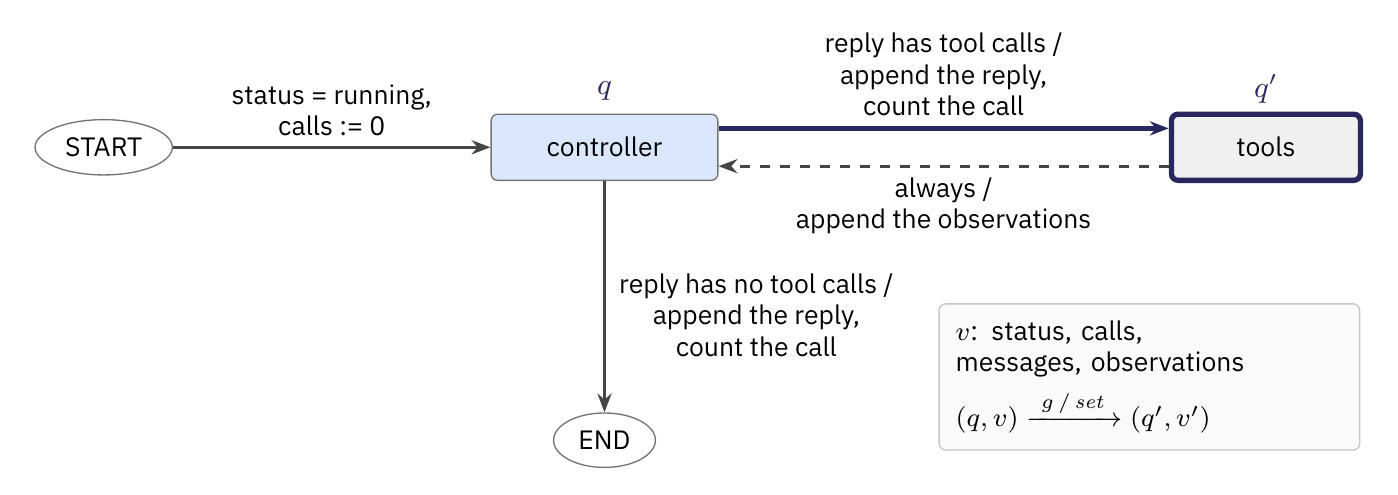
\includegraphics[width=0.8\textwidth]{figures/deck/fc6511c0f9.png}
  \caption{The two-node core of the planning version of \msa{}: the controller, which calls the
  model, and the tools node, which runs the requested tools. Each edge carries its guard and, after
  a slash, its set action, and the highlighted edge is one transition from $(q, v)$ to $(q', v')$.}
  \label{fig:recap-core}
\end{figure*}

A configuration pairs a control location $q$ with the values $v$ of the variables. The control
location is a node of the graph, such as the controller, and it names the computation that runs
next. The variables hold what the run keeps between steps, such as the messages exchanged with the
model and the number of model calls made so far.

Each edge of the graph is a transition. A transition is taken when its guard $g$ holds. The guard of
a transition is a true-or-false test of the variables and of the input that the step received, such
as the model's reply. When the transition is taken, its set action updates $v$. One step therefore
moves the run from a configuration $(q, v)$ to the next configuration $(q', v')$.

The state record stores the values $v$, one named field per variable. A node does not rewrite the
whole record. It returns a partial update, which holds new values only for the fields it changes.
The reducer of each field defines how the returned value is merged with the stored one. For example,
the reducer of \demoref{messages} appends the returned messages to the stored list, and the reducer
of \demoref{model\_calls}, the call count, adds each reported call to the stored total.

An invariant is a property that holds in every reachable configuration, that is, in every
configuration that some run can arrive at from its start. In the planning version, the call budget
gives an invariant: the count of completed model calls never exceeds the budget of 40. The property
holds because each node that calls the model, \demoref{plan}, \demoref{controller} and
\demoref{validate}, checks the count before the call and reports each completed call once.
Lecture~3 called this check the admission check.

Routing functions select the next node. A routing function is code that we write: after a node has
run, it reads the updated record and returns the name of the node that runs next.

A feedback edge sends the run back to a node that it visited earlier. The edge from the tools node
back to the controller, which Lecture~3 called the tool loop, is one example. Each feedback edge has
an explicit bound on how often a run can take it: a limit of its own or the call budget of the whole
run. In the planning version, the plan can be revised at most once per run. The call budget bounds
the other feedback edges, because each of them returns to the controller, which either ends the run
or calls the model.

A trace records one run. Its events show what the machine did, such as the model calls, the tool
requests and their results, and the routing decisions. When the run ends normally, a terminal event
states how it ended. Some moves between nodes have no event of their own and must be inferred.

The trace does not show what those actions did to the files or to anything else outside the
machine. The agent learns about the files only through what its tools report.

\Cref{fig:recap-core} draws the two-node core of the planning version, and the labels on its edges
show when each transition is taken and what it updates. The controller, drawn in blue, calls the
model, and the tools node, drawn in grey, runs the tools that the model requested. The full machine
also has the nodes \demoref{plan}, \demoref{submit} and \demoref{validate}. The figure leaves them
out and draws a reply without tool calls as the end of the run. In the full machine, such a reply
leads to \demoref{submit}, which checks the patch.

Each label gives the guard of the transition, then a slash, then its set action. The figure omits
the output actions, which Lecture~3 defined as the part of a transition that emits an output, such
as a request to run a tool. The arrow from \demoref{START} sets the status to \demoref{running} and
the call count to zero. The box at the bottom right lists the variables in $v$: the status, the call
count (written \emph{calls}), the messages and the observations.

The highlighted edge from the controller to the tools node is one transition from $(q, v)$ to
$(q', v')$. Its guard is that the model's reply has tool calls. Its set action appends the reply to
the messages and counts the call.

The edge from the controller to \demoref{END} has the opposite guard, that the reply has no tool
calls, and the same set action. The two guards exclude each other, because a reply either has tool
calls or has none. Exactly one of the two transitions is therefore taken after each model call.

The dashed edge from the tools node back to the controller is the tool loop. In the figure, its guard
always holds, and its set action appends the observations, the recorded results of the tool calls.

Lecture~3 drew the tools node as one box and treated everything that happens inside it as a single
step. This lecture opens that box, beginning with what a tool call is and which component executes
it (\cref{sec:toolcalls}).

\section{Tool calls}
\label{sec:toolcalls}

Lecture~3 drew the tools node of \msa{} as a single box (\cref{sec:recap}), and this section opens
it. We define a tool call, the harness that executes it and the boundaries that the call crosses, and
we follow the history of tool calling from remote procedure calls to the Model Context Protocol. The
history matters for design, because once a tool runs outside the harness's process, a call can fail
without a reply, and a retry can repeat its effect. The section ends with the terms that describe
such failures and with a design question about which component should prevent a repeated effect.

\subsection{What a tool call is}
\label{sec:toolcalls-what}

A tool call is a request that the model generates and another component executes. Lecture~2
introduced a tool call as a request to run one of the agent's tools, such as \demoref{read\_file},
with arguments. The model writes the request, and it never runs the tool itself.

The component that executes the request is the harness. The \textbf{harness} is the program that
runs the model loop and executes tool calls on the model's behalf. In \msa{}, the harness consists
of the graph that Lecture~3 studied and the dispatcher, the component that executes each tool call
(\cref{sec:dispatcher}). Lectures~2 and~3 called this program the runtime. From this lecture on, we
call it the harness.

Every tool call passes through the following operations, and each check on a call belongs to one of
them:
\be
\item \textbf{Find.} The harness finds the tool by its name. The name \demoref{edit}, for example,
selects the function that edits a file.
\item \textbf{Bind.} The harness binds the arguments to the parameters, matching each argument in
the request to a parameter of the tool's function.
\item \textbf{Check.} The harness checks \textbf{policy}, the rules that decide whether a requested
call is allowed. A rule might say, for example, that the agent may change only the files in its own
copy of the code.
\item \textbf{Run.} The tool runs and carries out the requested operation.
\item \textbf{Observe.} The harness observes the result and returns it to the model as an
observation, the tool's result as the harness records it (Lecture~2).
\ee
The model performs none of these operations. In this general description, the harness performs all
of them except running the tool. In \msa{}, the check that a path lies inside the agent's copy of
the code runs as the first step inside \demoref{read\_file} and \demoref{edit}, before either tool
touches a file. \Cref{sec:dispatcher} shows which component of \msa{} carries out each operation.

What a tool does, and what the harness must check, is written down in the tool's contract. A
\textbf{tool contract} is the written specification of a tool: what it does, which arguments it
accepts, its results and errors, its side effects and its execution constraints. A \textbf{side
effect} is a change that a call makes outside the caller, such as an edit to a file.
\Cref{sec:dispatcher} examines each part of a contract.

A tool call crosses two boundaries. A \textbf{boundary} is an interface that a request and its reply
cross. The first boundary lies between the model and the harness. The request leaves the model as
part of its reply, and the observation returns to the model as part of its next input. The second
boundary lies between the harness and the tool. The tool may be a function in the harness's own
process, or it may run in another process or on another machine.

Where the tool runs determines which guarantees a call has without extra code. When the tool is a
function in the harness's own process, calling it is a local call. A \textbf{local call} is a call
to a procedure in the caller's own process. If a local call returns, the tool ran, and it ran once.
If the tool fails, an exception reports why.

Across a process or machine boundary, the call loses these guarantees. The tool's contract and the
harness must then supply them explicitly. \Cref{sec:native} lists the guarantees of a local call,
and the history of tool calling (\cref{sec:toolcalls-history}) shows how a boundary takes them away.

\subsection{The history of tool calling}
\label{sec:toolcalls-history}

The history of tool calling divides into two periods: a pre-history before 2022 and a history that
begins around 2022. The pre-history concerns ordinary programs that call procedures on other
machines. The history concerns language models that request tools. The stages are the following:
\bi
\item \textbf{Before 2022.} Work on remote procedure calls, published in 1984 and 1994, established
that a remote call can fail in ways that a local call cannot (\cref{sec:toolcalls-rpc}).
\item \textbf{Around 2022.} Models wrote tool actions as text, and the harness parsed them. This
stage runs from WebGPT in December 2021 to ReAct in October 2022, and Toolformer, posted in
February 2023, also wrote its calls as text (\cref{sec:toolcalls-text}).
\item \textbf{2023 and 2024.} The model API began to return each call in a structured field of its
response, and later guaranteed that its arguments match a schema (\cref{sec:toolcalls-schemas}).
\item \textbf{Late 2024.} The Model Context Protocol moved the tool into its own process
(\cref{sec:toolcalls-mcp}).
\item \textbf{By 2026.} Studies measured how tool calls fail in real systems
(\cref{sec:toolcalls-studies}).
\ei

We describe each stage up to the Model Context Protocol by answering the following questions. What
could the caller or the model do? What did the interface promise? What still went wrong?
\Cref{tab:toolcalls-history}, at the end of \cref{sec:toolcalls-mcp}, collects the answers.

Remote procedure calls also introduced the problem that returns at the end of this history. A call
that crosses a boundary may fail without a reply, and its caller then cannot know whether the call
took effect.

\subsection{Remote procedure calls and partial failure}
\label{sec:toolcalls-rpc}

Remote procedure calls brought a way to fail that local calls do not have. A local call
(\cref{sec:toolcalls-what}) runs the procedure in the caller's own process. A \textbf{remote
procedure call} (\textbf{RPC}) is a call to a procedure on another machine, made to look like a
local call. The caller writes an ordinary call. The RPC system sends the arguments to the other
machine in a message, runs the procedure there, and returns its result to the caller in a reply.

The RPC system of 1984 promised \textbf{at-most-once semantics}, the guarantee that the effect of a
call happens zero times or once.

\begin{definition}[The call semantics of a remote procedure call]
\label{def:toolcalls-rpc}
``We guarantee that if the call returns to the user then the procedure in the server has been
invoked precisely once. Otherwise, an exception is reported to the user and the procedure will have
been invoked either once or not at all---the user is not told which.''
\citep[\S3.1]{birrell1984rpc}
\end{definition}

In the quotation, the user is the calling program, and the server is the machine that runs the
procedure. The guarantee has two halves. A call that returns ran the procedure exactly once. A call
that ends in an exception ran it at most once, and the caller does not learn whether it ran.

The same design prevented a resent message from running a procedure a second time. The
\textbf{transport} is the part of the system that carries messages between the machines. It resent
any message that might have been lost. Each call message carried an identifier for the call, and the
callee discarded any message whose identifier it had already seen.

This protection covers only the copies that the transport makes. Suppose the calling program
receives an exception and calls the procedure again. It then makes a new call with a new identifier,
and the callee runs it as a new call. A retry that the calling program issues is therefore a new
request.

What still went wrong was \textbf{partial failure}: one part of a system fails while the other parts
continue to run. Partial failure is one of the ways in which remote calls differ from local calls.
They also differ in latency, in memory access and in concurrency \citep[\S4]{waldo1994note}.

In a local call, the caller and the callee run in one process. A failure there either stops both of
them or reaches the caller as an exception. Across a boundary, the callee can crash, or a message
can be lost, while the caller keeps running. The caller then waits for a reply that never comes.

A lost request, a crashed callee and a lost reply all look the same to the caller: no reply arrives.
With no reply, the caller cannot tell whether the callee ran. \Cref{fig:toolcalls-local-remote}
contrasts the two kinds of call. In its right half, the callee has run, and only the reply is lost.

\begin{figure*}[t]
  \centering
  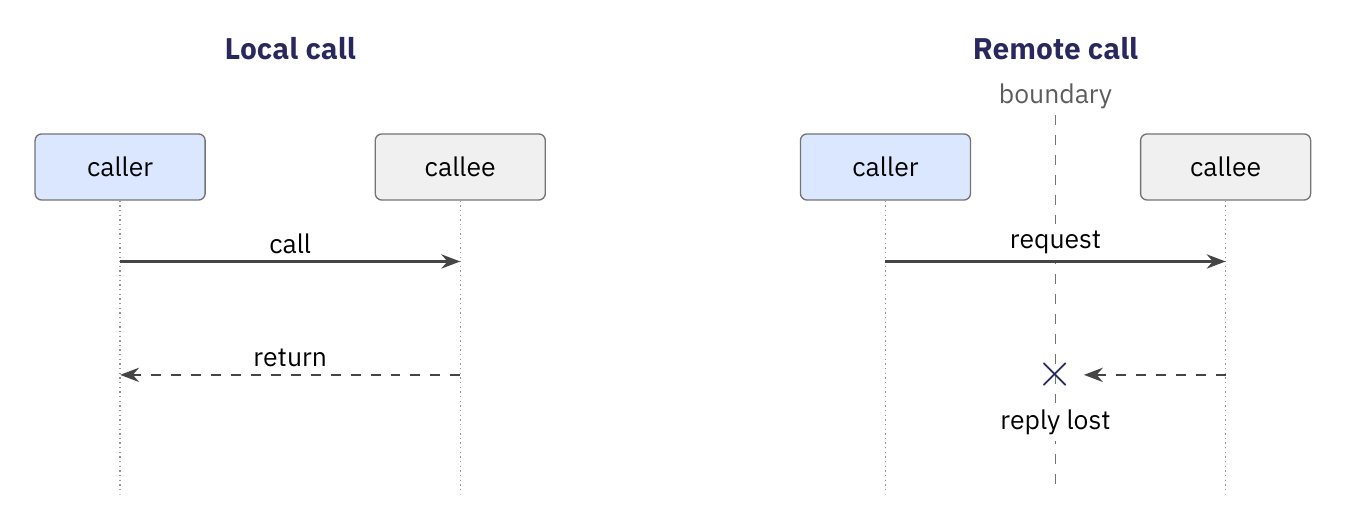
\includegraphics[width=0.7\textwidth]{figures/deck/300b345a5e.png}
  \caption{A local call and a remote call. In the local call, the callee's return reaches the
  caller. In the remote call, the request crosses a boundary and the callee runs, but its reply is
  lost, so the caller cannot tell whether the callee ran.}
  \label{fig:toolcalls-local-remote}
\end{figure*}

\subsection{Tool calls written as text}
\label{sec:toolcalls-text}

The first language models that used tools wrote their actions as ordinary text, and the harness had
to parse that text. WebGPT (December 2021) had the model issue commands to a text-based web browser
\citep{nakano2021webgpt}. MRKL systems (May 2022) routed text to separate tools
\citep{karpas2022mrkl}. ReAct (posted in October 2022 and presented at ICLR 2023) interleaved
reasoning with such actions \citep{yao2023react}. Toolformer, posted a few months later, in February
2023, trained a model to insert calls to APIs into its own text \citep{schick2023toolformer}.

Toolformer's model learned its call format in training. In ReAct, the prompt described the format.
In both systems, the call existed only as text, which the application had to find and parse. We call
the prompt-based form of this approach prompted calling. In \textbf{prompted calling}, the prompt
describes an action format, the model writes the action as text in that format, and the application
that called the model parses it. In our setting, that application is the harness.

\Cref{lst:toolcalls-react} shows an illustrative call in the style of ReAct. The model first writes
a thought, a passage of reasoning (Lecture~2). It then writes an action line, which names the tool
\demoref{edit} and gives its arguments in brackets. The harness finds the action line, splits it
into the tool's name and its arguments, runs the tool, and writes the result after
\texttt{Observation:}.

\begin{lstlisting}[float=tbp, basicstyle=\ttfamily\footnotesize, caption={An illustrative tool call written as text, in the style of ReAct.}, label=lst:toolcalls-react]
Thought: The loop bound in parse() is off by one.
Action: edit[src/parse.py, replace "i <= n" with "i < n"]
Observation: ok
\end{lstlisting}

The interface promised nothing. In prompted calling, the action format lived only in the prompt, and
nothing outside the prompt defined the call. Harnesses of this period typically found the action by
pattern matching. A pattern might, for example, look for a line that begins with \texttt{Action:}
and split the rest of that line at its brackets and commas.

What still went wrong was parsing. A malformed action line, such as one with a missing bracket or a
misspelled tool name, was rejected. An ambiguous action line was misread. Suppose the replacement text
in \cref{lst:toolcalls-react} itself contained a comma. A parser that splits the arguments at commas
would then cut the replacement in two and pass the wrong arguments to the tool. \Cref{sec:native}
returns to this example.

In this stage, the model, the prompt and the parser had to agree on a format that no interface
enforced.

\subsection{Tool schemas in the model API}
\label{sec:toolcalls-schemas}

In 2023 and 2024, the model API itself began to return tool calls in structured fields, and a schema
came to fix the shape of their arguments. OpenAI introduced this change in steps between June 2023
and August 2024.

In June 2023, the API began to return a call as a JSON object, separate from the text of the reply
\citep{openai2023functioncalling}. In \textbf{native tool calling}, the application's request to the
model API lists the available tools, and the response returns each call in its own structured field.
The request describes the arguments of each tool with a JSON Schema, a standard notation for the
names and types of the fields that a JSON object must have. The calling is native because the call
is part of the model API itself. OpenAI calls this function calling, and \cref{sec:native} studies it
in detail.

In November 2023, a single reply could contain several calls \citep{openai2023devday}.
\textbf{Parallel tool calls} are several tool calls in one reply, each with its own identifier. The
identifier lets the harness match each result to the call that it answers. The word parallel means
that the calls arrive together in one reply. The harness may still run them one after another
(\cref{sec:native}).

In August 2024, OpenAI added strict mode \citep{openai2024structuredoutputs}. \textbf{Strict mode} is
an option, set on each tool that the request lists, that guarantees that the arguments of each call
match the schema, within the subset of JSON Schema that strict mode supports. Before strict mode,
nothing in the API enforced the schema, and whether a call matched it was only a tendency of the
model. With strict mode, matching became a guarantee.

The vendor reports that, on its own evaluation of complex schema following, its new model of August
2024 with strict mode scored 100 percent, while an older model that relied on prompting alone scored
under 40 percent. This headline comparison changes the model and the method at once. The same post
also scores the new model with prompting alone and with strict mode off. Those results, rather than
the headline, show what strict mode adds on one model.

\Cref{lst:toolcalls-openai} shows an abbreviated call in OpenAI's chat format
\citep{openai-function-calling}. The call carries the identifier \texttt{call\_7}, the type
\texttt{function} and the name of the tool. Its arguments arrive as a string that contains JSON.
The application must parse that string before it can bind the arguments.

\begin{lstlisting}[basicstyle=\ttfamily\footnotesize, caption={An illustrative tool call in OpenAI's chat format, abbreviated. The arguments arrive as a string.}, label=lst:toolcalls-openai]
{ "id": "call_7",
  "type": "function",
  "function": {
    "name": "edit",
    "arguments": "{\"path\": \"src/parse.py\", ...}" } }
\end{lstlisting}

What still went wrong concerned the values of the arguments: a call can match its schema and still
name the wrong file. Suppose the off-by-one error lies in another file, and the model asks to edit
\texttt{src/parse.py}. The path is a string, as the schema requires, so the call is valid. The schema
guarantee covers the shape of the arguments: their names, their types and the fields that must be
present. It does not cover whether their values are right or what the call will do.

Both guarantees, that a call arrives in a structured field and that its arguments match the schema,
describe only the message that the API returns. The harness must still find the tool, bind the
arguments and check policy before the tool runs, and nothing in the API controls those steps.

\subsection{Tools in another process}
\label{sec:toolcalls-mcp}

In late 2024, the Model Context Protocol moved tools out of the harness's process. The
\textbf{Model Context Protocol} (\textbf{MCP}) is an open protocol that standardizes how a client
lists and calls the tools that a server offers in another process. Anthropic introduced it in
November 2024 \citep{anthropic2024mcp}. The \textbf{client} is the part of the harness that
exchanges messages with a server, and the \textbf{server} is a separate program that offers tools
and runs them. Lecture~5 studies MCP itself.

With MCP, the model could use any tool that a server listed. Every server describes its tools in the
same way, so a harness that implements MCP can use tools that were written without that harness in
mind.

The interface promised one standard for discovery, for the schemas of tool arguments, for results
and for errors. Discovery is the step in which the client asks a server which tools it offers.

In its current revision, the specification defines stdio and Streamable HTTP as its standard
transports, the ways in which
messages travel between the client and the server \citep{mcp-spec-2026-07-28}. Over stdio, the
server runs as a subprocess of the client, and messages travel over its standard input and output.
Over Streamable HTTP, the client sends each message to the server as an HTTP POST request. The reply
returns in the HTTP response, either as a single JSON object or as a stream of events.

MCP encodes every message in JSON-RPC, a standard format for remote calls written in JSON. A
JSON-RPC request names a method and carries an identifier that its reply repeats.
\Cref{lst:toolcalls-mcp} shows an abbreviated request. Its method, \texttt{tools/call}, asks the
server to call a tool. Its parameters name the tool, \demoref{edit}, and give the arguments. Its
id, 7, identifies the request, so that the client can match the reply to it. The request is
illustrative. The tools of \msa{} run in the harness's own process.

\begin{lstlisting}[basicstyle=\ttfamily\footnotesize, caption={An illustrative MCP request that calls the tool \texttt{edit}, abbreviated.}, label=lst:toolcalls-mcp]
{ "jsonrpc": "2.0",
  "id": 7,
  "method": "tools/call",
  "params": { "name": "edit", "arguments": { ... } } }
\end{lstlisting}

What still went wrong was the old problem of the RPC era. A call became a message, and a message can
be lost, delayed, or sent again by a retry. The harness can send this request and never learn
whether the server acted on it. This is the partial failure of \cref{sec:toolcalls-rpc}. It returns
as soon as the tool leaves the harness's process.

\Cref{tab:toolcalls-history} summarizes the stages of the history with the questions of
\cref{sec:toolcalls-history}. Its last column shows how the main failure changed from one stage to
the next. Text actions failed at parsing. Calls returned under a schema could still carry wrong
values, because the schema covers only their shape. Moving tools into separate processes brought
back the partial failure of remote procedure calls.

\begin{table*}[t]
  \caption{The stages of the history of tool calling: what the caller or the model could do, what
  the interface promised, and what still went wrong.}
  \label{tab:toolcalls-history}
  \begin{adjustbox}{width=\linewidth}\begin{tabularx}{\linewidth}{L{0.19\linewidth}XXX}
    \toprule
    \textbf{Stage} & \textbf{What the caller or the model could do} & \textbf{What the interface
    promised} & \textbf{What still went wrong} \\
    \midrule
    \textbf{Remote procedure calls (1984 and 1994)} & A program could call a procedure on another
    machine as if the call were local. & At-most-once semantics: a call that returns ran the
    procedure once, and an exception means once or not at all. & Partial failure: when no reply
    arrives, the caller cannot tell whether the callee ran. \\ \addlinespace
    \textbf{Text actions (2021 to early 2023)} & The model could write an action as text, which the
    harness parsed. & Nothing: the action format lived only in the prompt. & Parsing: a malformed or
    ambiguous action line was rejected or misread. \\ \addlinespace
    \textbf{Schemas in the model API (2023 and 2024)} & The model could return a call as JSON, and
    several calls in one reply, each with an identifier. & Each call arrives in its own structured
    field (2023). With strict mode (2024), its arguments match the schema. & Wrong values: a call can match the schema
    and still name the wrong file. \\ \addlinespace
    \textbf{Tools in another process (MCP, from 2024)} & The model could use any tool that a server
    listed. & One standard for discovery, schemas of tool arguments, results and errors, over stdio
    and, in the current revision, Streamable HTTP. & The problem of the RPC era: a message can be lost, delayed, or sent again
    by a retry. \\
    \bottomrule
  \end{tabularx}\end{adjustbox}
\end{table*}

\subsection{Studies of tool-call failures}
\label{sec:toolcalls-studies}

By 2026, studies had begun to measure how tool calls fail in real systems. They include fault
catalogs, injected-fault benchmarks and a study of checkpoint-restore:
\bi
\item \textbf{Fault catalogs.} A fault catalog classifies the failures found in real software. Two
studies of 2026 grouped real failures of MCP software into named categories
\citep{taraghi2026mcpfaults,owotogbe2026mcpruntime}.
\item \textbf{Injected-fault benchmarks.} A benchmark of this kind makes tools fail on purpose
during a run, for example by letting them time out, limit the rate of requests or return partial
results. A benchmark of January 2026 measured how far the success of agents falls under such faults
\citep{gupta2026reliabilitybench}.
\item \textbf{A study of checkpoint-restore.} A checkpoint saves a run's progress so that the run can
resume from that point (Lecture~2). Agent frameworks that offer checkpoint-restore advise developers
to make tool calls safe to retry. A study of March 2026 examined whether this advice prevents
duplicate effects at the tool boundary \citep{zheng2026acrfence}. After a restore, the agent
regenerates its requests, and they differ slightly from the original ones. Servers treat them as new
requests, so irreversible effects, such as a payment, can happen again.
\ei
Together, these studies treat failures at the tool boundary, including timeouts and repeated
effects, as events that can be observed, classified and measured.

\subsection{A retried request}
\label{sec:toolcalls-retry}

A retried request can apply the same patch twice. Consider a harness that calls a tool on an MCP
server, and suppose that the tool applies a patch to a file. \Cref{fig:toolcalls-retry} draws the
exchange with time running downward. On the server's side, it shows the patch applied once for the
request with id 7 and again for the request with id 8. The scenario unfolds as follows:
\bi
\item \textbf{The request.} The request with id 7 reaches the server, and the server applies the
patch.
\item \textbf{The reply.} The reply never reaches the harness. After waiting for a set time, the
harness gives up, and the request has timed out. The harness cannot tell whether the patch was
applied.
\item \textbf{The retry.} The harness sends the request again. The retry is a new request with id 8,
and the server applies the patch a second time.
\ei

\begin{figure*}[t]
  \centering
  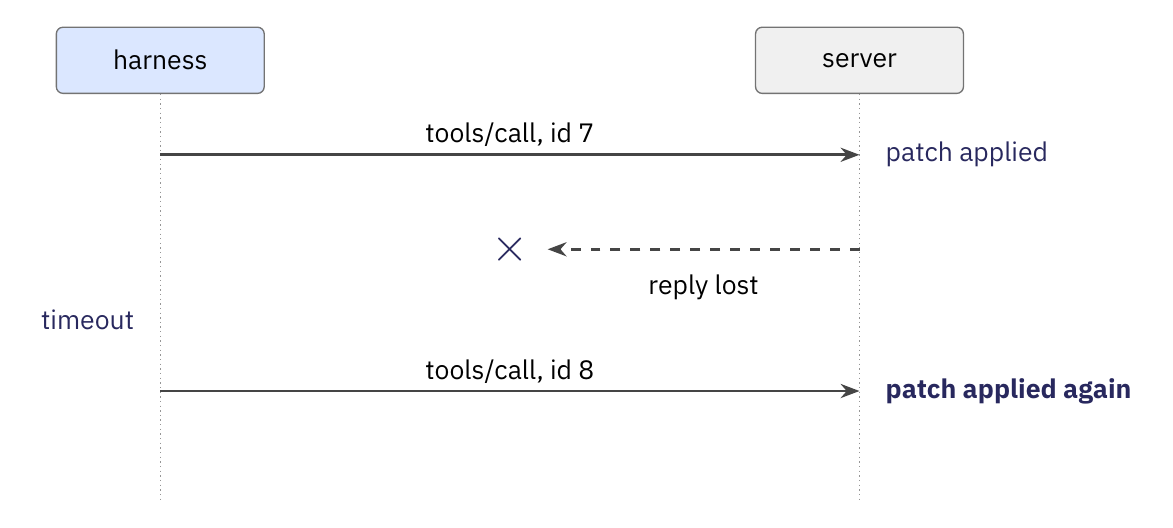
\includegraphics[width=0.6\textwidth]{figures/deck/a9a99892bc.png}
  \caption{A retried request applies the same patch twice. The server applies the patch for the
  request with id 7, but its reply is lost. The harness times out and sends the request again with
  id 8, and the server applies the patch again.}
  \label{fig:toolcalls-retry}
\end{figure*}

Nothing in MCP lets the server recognize the retry. The relevant rules of MCP, in its revision
2026-07-28, are the following \citep{mcp-spec-2026-07-28}:
\bi
\item \textbf{A broken stream cannot be resumed.} Over Streamable HTTP, a reply that the server
streams travels on a response stream, the open HTTP response that carries the server's messages for
that one request. A stream that breaks cannot be resumed, so a reply lost with it cannot be fetched
again.
\item \textbf{Closing the stream cancels the request.} Over Streamable HTTP, the server must treat
the client's closing of the response stream as a cancellation of the request. The server may
already have finished the work when the cancellation arrives.
\item \textbf{The id matches replies to requests.} A request's id must differ from the id of every
request that is still awaiting its reply. The id tells the client which reply answers which request.
It does not tell the server that a request repeats an earlier one.
\item \textbf{No field marks a repeat.} The core protocol has no field that marks a request as a
repeat of another.
\ei
A retry is therefore a separate request with its own id. The server cannot tell it from a first
request, so it runs the tool again.

From the harness's side, both choices after a missing reply carry a risk. With no reply, the harness
cannot tell a lost request from a lost reply. If it does not retry and the request was lost, the
patch is never applied. If it retries and the reply was lost, the patch is applied twice.

\subsection{Terms for calls across a boundary}
\label{sec:toolcalls-terms}

The scenario of \cref{sec:toolcalls-retry} can be stated precisely with the terms below. They build
on two terms of \cref{sec:toolcalls-what}: the harness, which runs the model loop and executes tool
calls, and a boundary, an interface that a request and its reply cross. Across a process or machine
boundary, a function call becomes a message that can be lost, delayed or delivered twice.

The semantics of a call states how many times its side effect occurs. Under at-most-once semantics
(\cref{sec:toolcalls-rpc}), the effect occurs zero times or once. Under \textbf{at-least-once
semantics}, it occurs one or more times. Under \textbf{exactly-once semantics}, a side effect occurs
once despite lost requests, lost replies or duplicate delivery. \Cref{tab:toolcalls-semantics}
compares these semantics, and its last column gives the risk under each when no reply arrives.

\begin{table}[htbp]
  \caption{Semantics of a call that crosses a boundary: how often the effect occurs, and the risk
  when no reply arrives.}
  \label{tab:toolcalls-semantics}
  \begin{adjustbox}{width=\linewidth}\begin{tabularx}{\linewidth}{L{0.25\linewidth}L{0.24\linewidth}X}
    \toprule
    \textbf{Semantics} & \textbf{The effect occurs} & \textbf{Risk when no reply arrives} \\
    \midrule
    \textbf{At-most-once} & Zero times or once & A missing effect, when the caller does not retry
    and the request was lost \\ \addlinespace
    \textbf{At-least-once} & One or more times & A repeated effect, when the caller retries and only
    the reply was lost \\ \addlinespace
    \textbf{Exactly-once} & Once & Neither a missing nor a repeated effect, provided that a repeated
    request has no further effect \\
    \bottomrule
  \end{tabularx}\end{adjustbox}
\end{table}

A harness that never retries obtains at-most-once semantics. A harness that retries until it
receives a reply obtains at-least-once semantics, and the scenario of \cref{sec:toolcalls-retry}
shows the cost: the patch was applied twice. Exactly-once semantics needs both a retry and a
receiver for which a repeated request has no further effect.

A repeated request has no further effect in two cases. In the first, the request is idempotent. An
\textbf{idempotent request} has the same effect when repeated as when executed once. In \msa{},
requests to \demoref{read\_file} and \demoref{search} are idempotent, because these tools only read
files, so repeating them changes nothing. The patch request of the scenario is not idempotent,
because each execution applies the patch again.

In the second case, the receiver recognizes the repeat. An \textbf{idempotency key} is an identifier
that a request carries so that the receiver can detect a duplicate and avoid repeating its effect.
The original request and every retry of it carry the same key. A receiver that remembers the keys it
has processed can then decline a request whose key it has already seen.

The request id of \cref{lst:toolcalls-mcp} cannot serve as an idempotency key, because a retry
carries a new id. The identifier that the RPC system of 1984 attached to each call served this
purpose, but only for the copies that its transport made (\cref{sec:toolcalls-rpc}).

\subsection{Which component should prevent a repeated patch}
\label{sec:toolcalls-question}

The scenario raises a design question. The harness sends a request that applies a patch and
receives no reply. Which component is responsible for ensuring that the patch is applied once?

The duty could fall to the model, which can check the state of the file before it asks for the
patch again. It could fall to the harness, which decides whether to retry. It could fall to the tool
contract, which can accept a key that marks a repeat. In the scenario as described, no component
holds it.

Any answer must respect the following facts:
\bi
\item \textbf{A missing reply is ambiguous.} The absence of a reply does not distinguish a lost
request from a lost reply (\cref{sec:toolcalls-retry}).
\item \textbf{Retries create duplicates.} Any component that retries must therefore allow for
duplicate requests.
\item \textbf{A key lets the receiver decline.} An idempotency key in the tool's contract is the
mechanism that lets the receiver recognize a duplicate and decline it
(\cref{sec:toolcalls-terms}).
\ei

The question is an instance of a broader one: which component enforces a given guarantee?
\Cref{sec:dispatcher} asks it for each guarantee that the harness of \msa{} provides.

\subsection*{Key points}
\bi
\item A tool call is a request that the model generates and the harness executes: the harness finds
the tool by name, binds the arguments and checks policy, the tool runs, and the harness returns the
observed result to the model.
\item A tool call crosses two boundaries, model to harness and harness to tool, and once the tool
runs outside the harness's process, the contract and the harness must supply the guarantees of a
local call explicitly.
\item Remote procedure calls promised at-most-once semantics, but under partial failure a caller
that receives no reply cannot tell whether the callee ran.
\item Prompted calling defined the call only in the prompt, so the harness had to parse actions from
text and could reject or misread them.
\item Native tool calling returns each call in a structured field, and strict mode guarantees only
the shape of its arguments, so the harness must still find, bind and check the call before the tool
runs.
\item MCP moved tools into separate server processes, so a call became a message that can be lost,
and a retry carries a new id that the server cannot recognize as a repeat.
\item Any component that retries must allow for duplicate requests, and exactly-once semantics needs
a repeated request to have no further effect, either because the request is idempotent or because an
idempotency key lets the receiver decline it.
\ei

\section{The tool dispatcher}
\label{sec:dispatcher}

\Cref{sec:toolcalls} described a tool call as five operations of the harness: it finds the tool,
binds the arguments, checks policy, runs the tool and observes the result. In \msa{}, one component
of the harness, the dispatcher, carries out these operations or calls the code that does. It finds
the tool, binds the arguments and records the observation itself, and the tool function that it
calls checks the path and performs the operation. This section explains what a tool contract
specifies, how the dispatcher executes one call, which record shows that a tool ran, and which
component enforces each guarantee of the harness, that is, each property that the harness promises
for every run, such as that only registered tools run. These questions matter because the model's
requests reach the files only through the dispatcher, so a guarantee holds only where code on that
route checks it.

The dispatcher also carries out the dispatch and observe steps of the reactive loop of Lecture~2, in
which the harness checks and executes each tool call and then records its result. The Lecture~2
notes left the details of that check to this lecture.

\subsection{What a tool contract specifies}
\label{sec:dispatcher-contract}

A tool contract is the written specification of a tool (\cref{sec:toolcalls}). It specifies the
following:
\bi
\item \textbf{Purpose.} The contract states what the tool does, for example that it reads a file or
replaces a string in a file.
\item \textbf{Arguments.} The contract lists the arguments the tool accepts, with their names, their
types and any constraints on their values.
\item \textbf{Results and errors.} The contract states what a successful call returns and how a
failed call is reported.
\item \textbf{Side effects.} The contract states the changes a call makes besides returning its
result, such as changes to files.
\item \textbf{Execution constraints.} The contract limits where and how the tool may operate, for
example by requiring that every file the tool writes lies inside the run's own copy of the code
base (\cref{sec:dispatcher-role}).
\ei

The model receives only part of the contract. A \textbf{tool definition} is the part of the
contract that the model receives: the tool's name, a description of its purpose, and an
\textbf{argument schema}. The argument schema gives the names and types of the arguments and the
constraints on them. The rest of the contract, namely the results, errors, side effects and
execution constraints, is defined by the tool's implementation and by the dispatcher.

This division determines where a constraint can be enforced. A description is text that the model
reads. It can state a rule, but nothing in the text stops a call that breaks the rule. A constraint
holds only when code checks it, in the implementation of the tool or in the dispatcher. A
description alone therefore enforces nothing.

The tools of \msa{} differ in their side effects:
\bi
\item \textbf{\demoref{read\_file}.} The tool returns the text of a file, or of a range of its
lines.
\item \textbf{\demoref{search}.} The tool returns the lines that match a regular expression, each
with its file and line number. An optional \textbf{glob}, a file pattern with wildcards such as
\texttt{src/*.py}, selects the files to search.
\item \textbf{\demoref{edit}.} The tool replaces one exact string in a file with another. It is the
only tool that writes files.
\ei
\demoref{read\_file} and \demoref{search} only read. Every tool function takes as its first
parameter the path of the run's copy of the code base, and the dispatcher supplies that value
(\cref{sec:dispatcher-binding}).

\subsection{The dispatcher}
\label{sec:dispatcher-role}

The \textbf{dispatcher} is the harness component that receives each tool request, the tool call as
the tools node passes it on, executes it against the workspace and returns an observation to the
model. The \textbf{workspace} is a disposable copy of the code base that one run may read and edit.
It holds the files of the pinned commit of Lecture~2, the fixed version of the code base from which
every run begins. It plays the role of the working tree of Lecture~2, the copy of the files that the
agent reads and edits during a run. The \textbf{workspace root} is the path of that copy.

The dispatcher holds the registry, the workspace root and the trace, and the model never touches any
of them. The \textbf{registry} is the table that maps each tool name to the function that
implements the tool. The trace is the log of events that the harness writes during a run
(Lecture~2).

\Cref{fig:dispatcher-role} shows where the dispatcher sits between the model and the files. The
tools node of \msa{} calls the dispatcher once for each tool call in the model's reply. The
dispatcher looks the tool up in the registry, binds the arguments, and calls the tool function with
the workspace root that it holds. It writes a \demoref{tool\_request} event and a
\demoref{tool\_result} event to the trace. It then returns an observation, which the tools node turns
into a tool message. A \textbf{tool message} is the message that carries one tool result back to the
model.

\begin{figure*}[t]
  \centering
  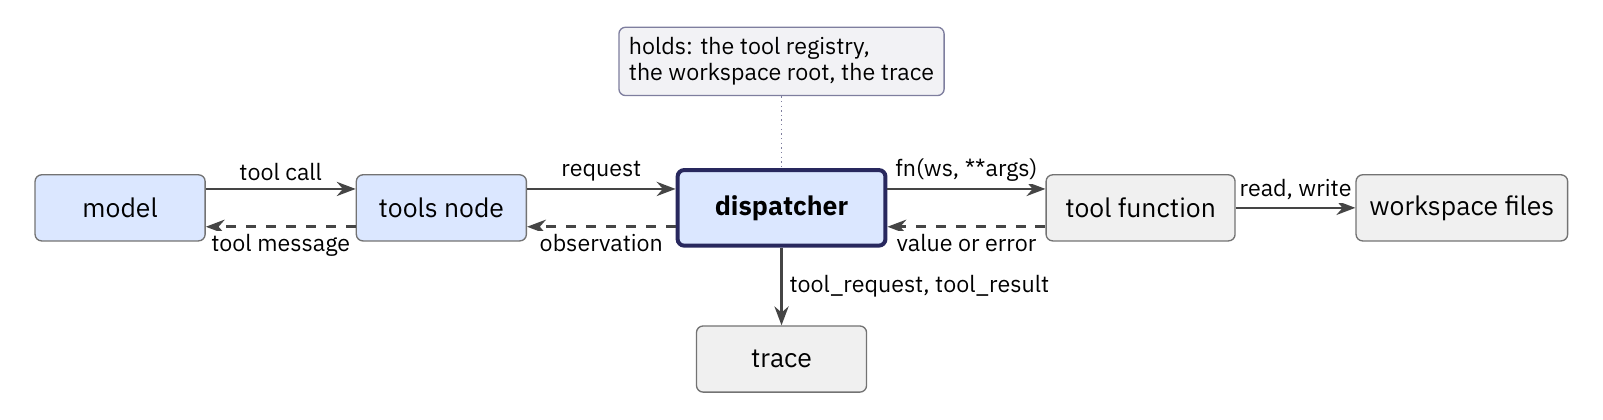
\includegraphics[width=0.9\textwidth]{figures/deck/d9c53fb5c2.png}
  \caption{The dispatcher between the tools node and the tool function. The dispatcher calls the
  tool function with the workspace root and the model's arguments, writes two events to the trace,
  and returns an observation, which reaches the model as a tool message. Only the tool function
  reads or writes the workspace files.}
  \label{fig:dispatcher-role}
\end{figure*}

The model never calls a tool function. It can only request a call, by writing a tool call in its
reply. The dispatcher decides whether the call runs and how. Whatever the model writes, a tool
function runs only when the dispatcher calls it, so every check placed in the dispatcher applies to
every tool call.

\subsection{Binding and the workspace root}
\label{sec:dispatcher-binding}

The dispatcher supplies the workspace root itself and lets the model supply only the other
arguments. \textbf{Binding} is the step that matches the model's arguments to the parameters of the
tool function without calling the function. The dispatcher binds the workspace root to the first
parameter, \demoref{ws}, and matches the model's arguments by name to the parameters that remain.
\Cref{lst:dispatcher-bind} shows the signature of \demoref{read\_file} and the call that performs
the binding.

\begin{lstlisting}[float=tbp, basicstyle=\ttfamily\footnotesize, caption={Illustrative code: the signature of \demoref{read\_file}, and the call with which the dispatcher binds the model's arguments to it.}, label=lst:dispatcher-bind]
def read_file(ws: Path, path: str,
              start: int | None = None,
              end: int | None = None) -> str: ...

# the dispatcher supplies ws before the model's arguments
inspect.signature(function).bind(ws, **args)
\end{lstlisting}

The function \demoref{read\_file} takes the workspace root \demoref{ws}, the path of a file, and an
optional range of lines from \demoref{start} to \demoref{end}. In the last line, \demoref{function}
is the function that the registry returned for the requested name, and \demoref{args} holds the
arguments of the model's tool call. Python's \demoref{inspect.signature(...).bind} checks that a set
of arguments fits a function's parameters, and it does not call the function. If a name matches no
parameter, or a required parameter receives no value, binding fails and the dispatcher refuses the
request. A \textbf{refusal} is the dispatcher's decision not to run a request. The dispatcher
returns the reason to the model as an observation instead, and the run continues
(\cref{sec:dispatcher-refusals}).

A request that names \demoref{ws} fails to bind, because the dispatcher has already supplied that
parameter. The model therefore cannot replace the root against which the tools resolve their paths.
The argument schema also omits \demoref{ws}, so the model is never told that the parameter exists.
The model still chooses the path arguments, so a tool that opens a path must still check it
(\cref{sec:dispatcher-search}).

Binding also explains why the tools read the run's settings, such as its limits, from a module.
Every parameter after the workspace root is a value the model may supply. If a tool took the run's
settings as a parameter, for example a parameter named \demoref{config}, binding would accept a
value for it from the model like any other argument. No argument from the model can reach a value
that the tool reads from a module.

Both choices follow one principle. \textbf{Authority} is the power to decide something about the
run, such as which directory a tool may touch or which limits apply. The model cannot supply
authority it was never given, because the harness supplies those values itself, outside the reach
of the model's arguments.

\subsection{What the model sees and what runs}
\label{sec:dispatcher-definition}

The model sees a tool's definition, and the dispatcher runs the tool's function. The definition
describes the tool's rules, and only the function and the dispatcher's checks enforce them. In
\msa{}, the definition of \demoref{edit} is written as a
separate function, \demoref{edit\_schema}, whose name, parameters and description are converted
into the definition that the model receives. Its body never runs. The dispatcher executes the real
\demoref{edit} instead, so that every call passes through the dispatcher's checks and appears in the
trace.

\Cref{lst:dispatcher-schema} shows the definition of \demoref{edit} in the JSON form in which the
model receives it. The \demoref{description} field states the tool's purpose and its rules. The
\demoref{parameters} field is the argument schema: it lists three required string arguments,
\demoref{path}, \demoref{old} and \demoref{new}. It omits \demoref{ws}, which the dispatcher
supplies. Model providers use slightly
different formats for the same content (\cref{sec:native}).

\begin{lstlisting}[float=tbp, basicstyle=\ttfamily\footnotesize, caption={Illustrative code: the definition of \demoref{edit} as the model receives it, abbreviated.}, label=lst:dispatcher-schema]
{"type": "function",
 "function": {
   "name": "edit",
   "description": "Replace an exact string in a
     file. `old` must appear exactly once in the
     file, so include enough surrounding text to
     make it unique. ...",
   "parameters": {
     "type": "object",
     "properties": {
       "path": {"type": "string"},
       "old":  {"type": "string"},
       "new":  {"type": "string"}},
     "required": ["path", "old", "new"]}}}
\end{lstlisting}

The description tells the model that \demoref{old} must occur exactly once in the file. Only the
body of \demoref{edit} enforces that rule (\cref{lst:dispatcher-edit}). The function counts the
occurrences of \demoref{old} and raises an error, before it writes anything, unless the count is
exactly one. If the sentence were deleted from the description, the rule would still hold. If the
count were deleted from the body, the rule would no longer hold, whatever the description said.

\begin{lstlisting}[float=tbp, basicstyle=\ttfamily\footnotesize, caption={Illustrative code: an excerpt of the function \demoref{edit} that the dispatcher runs.}, label=lst:dispatcher-edit]
def edit(ws, path, old, new):
    target = resolve(ws, path)    # the path check
    body = target.read_text()
    occurrences = body.count(old)
    if occurrences != 1:
        raise ValueError(...)     # nothing written
    target.write_text(body.replace(old, new, 1))
    return {"path": path, "replaced": 1}
\end{lstlisting}

The first line of the body is the path check. The \textbf{path check} accepts a path only if it
resolves to a location inside the workspace root, and raises an exception otherwise. To resolve a
path is to rewrite it as the absolute location it names, so that a step up to a parent directory,
written \texttt{..}, is applied before the comparison. In \msa{}, the path check is the function
\demoref{workspace.resolve}. It is the first step of \demoref{read\_file} and of \demoref{edit}.

\subsection{The dispatch cycle}
\label{sec:dispatcher-cycle}

Each tool call passes through a cycle of operations that the dispatcher controls
(\cref{fig:dispatcher-cycle}):
\be
\item \textbf{Find.} The dispatcher looks the tool's name up in the registry. A name that is not
registered is refused.
\item \textbf{Bind.} The dispatcher binds the arguments to the function's parameters
(\cref{sec:dispatcher-binding}). Arguments that do not bind are refused.
\item \textbf{Check.} The request is checked against the policy. In \msa{}, the policy requires
every path to lie inside the workspace root. The path check enforces it as the first step inside
\demoref{read\_file} and \demoref{edit}, and a path outside the root is refused. A call to
\demoref{search} passes through no such check (\cref{sec:dispatcher-search}).
\item \textbf{Run.} The tool function performs the permitted operation. It returns a value, or it
fails with an error.
\item \textbf{Observe.} The dispatcher records the outcome as an observation and writes a
\demoref{tool\_result} event to the trace. An observation carries the \demoref{ok} flag, the result
or the reason for a failure, and the arguments of the call. The \demoref{ok} flag is true only when
the call succeeded.
\ee

\begin{figure}[htbp]
  \centering
  \begin{adjustbox}{width=\linewidth}
  \begin{tikzpicture}[node distance=4mm,
      op/.style={rnode, text width=41mm, align=left}]
    \node[tnode] (req) {tool request};
    \node[op, below=of req] (find) {\textbf{find} the tool's name in the registry};
    \node[op, below=of find] (bind) {\textbf{bind} the arguments to the function's parameters};
    \node[op, below=of bind] (check) {\textbf{check} that the path lies inside the workspace root};
    \node[op, below=of check] (run) {\textbf{run} the permitted operation};
    \node[op, below=7mm of run, fill=ibmblue!15] (obs) {\textbf{observe}: an observation with
      \texttt{ok}, the result or the reason, and the arguments};
    \node[tnode, below=of obs] (out) {state record, trace event, next model input};
    \draw[flow] (req) -- (find);
    \draw[flow] (find) -- (bind);
    \draw[flow] (bind) -- (check);
    \draw[flow] (check) -- (run);
    \draw[flow] (run) -- node[lab, right=1mm] {result, or error} (obs);
    \draw[flow] (obs) -- (out);
    \coordinate (bus) at ([xshift=-27mm]find.west);
    \draw[back] (find.west) -- node[lab, above=0.5mm] {unregistered tool} (find.west -| bus)
      |- (obs.west);
    \draw[thick, dashed, draw=ibmfg!80] (bind.west) -- node[lab, above=0.5mm]
      {arguments do not bind} (bind.west -| bus);
    \draw[thick, dashed, draw=ibmfg!80] (check.west) -- node[lab, above=0.5mm]
      {path outside the root} (check.west -| bus);
  \end{tikzpicture}
  \end{adjustbox}
  \caption{The dispatch cycle for one tool request. The solid arrows are the path of a permitted
  call. The dashed arrows are the refusals of an unregistered tool, of arguments that do not bind
  and of a path outside the root, and they end in an observation, as a permitted call does.}
  \label{fig:dispatcher-cycle}
\end{figure}

\Cref{lst:dispatcher-cycle} writes the cycle as pseudocode. The comments mark the operations.

\begin{lstlisting}[float=tbp, basicstyle=\ttfamily\footnotesize, caption={Illustrative pseudocode for the dispatch of one tool request.}, label=lst:dispatcher-cycle]
def dispatch(request):
    trace.event("tool_request", request)
    fn = registry.get(request.name)     # find
    if fn is None:
        return refuse("unregistered tool")
    try:
        bind(fn, ws, request.args)      # bind
    except TypeError:
        return refuse("bad arguments")
    try:                                # check + run
        value = fn(ws, **request.args)
    except PathEscape:
        return refuse("outside workspace")
    return observe(value)               # observe
\end{lstlisting}

The listing makes the order of events explicit:
\bi
\item \textbf{The request event.} The first line writes the \demoref{tool\_request} event before any
check, so every request appears in the trace, including the requests that are later refused.
\item \textbf{Find and bind.} A name missing from the registry, or arguments that do not bind, end
the dispatch with a refusal before any tool function is called. Binding signals a mismatch by
raising Python's \demoref{TypeError}.
\item \textbf{Check and run.} The tool function is called with the workspace root and the model's
arguments. \demoref{PathEscape} stands for the exception that the path check raises.
\item \textbf{Refuse and observe.} Each of \demoref{refuse} and \demoref{observe} writes a
\demoref{tool\_result} event and returns an observation. A refusal carries \demoref{ok} false and the
reason. A successful call carries \demoref{ok} true and the result.
\ei
The listing omits the conversion of argument types and the handling of failures inside a tool,
which \cref{sec:dispatcher-refusals} describes.

In \msa{}, the check of policy is not a separate stage of the dispatcher. It is the path check, the
first step inside \demoref{read\_file} and \demoref{edit}. When a path lies outside the root, the
path check raises its exception before the tool reads or writes anything, and the dispatcher turns
that exception into a refusal. For this reason the check and the run share one \texttt{try} block
in the listing, while \cref{fig:dispatcher-cycle} draws them as separate boxes.

Every request ends in an observation, unless an exception that the dispatcher does not expect
interrupts the cycle. Such an exception ends the run without an observation
(\cref{sec:dispatcher-refusals}). The harness stores each observation in the state record
(Lecture~3), and the model reads it in its next input.

\subsection{Refusals}
\label{sec:dispatcher-refusals}

A refused call returns an error to the model as an observation, and the run continues. The
observation of a refusal (\cref{sec:dispatcher-binding}) has its \demoref{ok} flag set to false,
and its result states the reason.

A harness can report a failed call as an exception or as an observation, and the two affect the run
differently:
\bi
\item \textbf{An exception.} An unhandled exception ends the run.
\item \textbf{An observation.} An observation reaches the model, which reads what went wrong and can
revise its request, for example by correcting an argument name or choosing a path inside the
workspace.
\ei
The reactive loop of Lecture~2 depends on observations. The loop works because the model sees the
result of each action, and a refusal is a result that the model can act on.

A \textbf{tool error} is a failure of the tool's operation itself, after the request has passed the
checks. An \demoref{edit} whose \demoref{old} string occurs twice is an example. The operation
cannot tell which occurrence to replace, so the function raises an error before it writes anything
(\cref{sec:dispatcher-definition}). The dispatcher catches the tool errors it expects and returns
each one as an observation with \demoref{ok} false, as it does for a refusal.

A refusal and a tool error differ in what failed. A refusal comes from a check of the request: the
name is not registered, the arguments do not bind, or a path lies outside the workspace root. A
tool error comes from the operation, which could not be carried out on the files as they are. In
\msa{}, the path check and the operation both run inside the tool function. A failed path check
still counts as a refusal, because it checks the request and fails before the tool opens any file.

Binding checks the names of the arguments and their number. It does not check their types. When a
type mismatch is unambiguous, the dispatcher converts the value instead of refusing the request.
This conversion is called \textbf{coercion}. If the model passes the string \texttt{"40"} where the
function expects an integer, the dispatcher converts it to the integer 40. A refusal would spend a
model call only to tell the model that its string should have been a number.

The dispatcher catches only the exceptions it expects, and any other exception ends the run. The
design intends this for failures from which the run cannot recover, such as a trace that cannot be
written. An unexpected exception raised inside a tool also ends the run. For example, the library
that \demoref{search} uses to expand a glob raises an exception when the glob is an absolute path.
The dispatcher does not expect this exception, so the run ends and the model never receives a
refusal.

A \textbf{precondition} is a condition that must be true before a call, for example that
\demoref{old} occurs exactly once in the file. A contract that states only its preconditions leaves
the outcome of a wrong request undefined, as the glob example shows. The contract must also say
what happens when a request violates a precondition: whether the call returns a refusal or a tool
error that the model can read, or raises an exception that ends the run.

\subsection{What each record establishes}
\label{sec:dispatcher-records}

A tool call leaves several records, and each establishes something different about whether the
tool ran. The trace of \msa{} records a \demoref{model\_call} event when a node calls the model, a
\demoref{routing} event after each reply of the controller, when its routing function chooses
between the tools node and \demoref{submit}, and the dispatcher's \demoref{tool\_request} and
\demoref{tool\_result} events. Some moves, such as the return from the tools node to the controller,
have no event of their own (\cref{sec:recap}). \Cref{tab:dispatcher-records} follows one
\demoref{read\_file} call of \msa{}, in which the model reads the file that the alert flags. Its rows run from the model's input to the next model
input, in the order in which the records arise. The rows to compare are the model's response and
the \demoref{tool\_result} event.

\begin{table}[htbp]
  \caption{The records that one \demoref{read\_file} call leaves, in the order in which they arise,
  and what each establishes about the execution of the tool.}
  \label{tab:dispatcher-records}
  \begin{adjustbox}{width=\linewidth}\begin{tabularx}{\linewidth}{@{}L{0.3\linewidth}X@{}}
    \toprule
    \textbf{Record or stage} & \textbf{What it establishes} \\
    \midrule
    \textbf{Model input} & The input contains the available tool definitions. The trace does not
      record this input. \\
    \textbf{Model response and \demoref{model\_call} event} & The model asked to call a tool. The
      request alone does not establish that the tool ran. \\
    \textbf{\demoref{routing} event} & The run went to the tools node because the reply contained a
      tool call. The event records a decision and says nothing about execution. \\
    \textbf{\demoref{tool\_request} event} & The dispatcher received the request and began checking
      it. \\
    \textbf{Dispatcher} & The dispatcher checked the request. A refusal reason appears in
      \demoref{tool\_result}, and no separate event is written for each check. \\
    \textbf{\demoref{tool\_result} event} & With \demoref{ok} true, the function ran and returned.
      The event records the length of the result and omits its text. \\
    \textbf{State and next input} & The harness stores the observation in the state record and adds
      a tool message to the next model input. \\
    \bottomrule
  \end{tabularx}\end{adjustbox}
\end{table}

Between the model's response and the execution of the tool lie the dispatcher's checks, and any of
them could have refused the request. The dispatcher writes a successful \demoref{tool\_result} event
only after the function has returned.

The routing event lies between the model's response and the \demoref{tool\_request} event. As in
Lecture~2, a routing event records one routing decision, and its \demoref{by} field names who
supplied the value that the routing function tested. Here the event records that the run went to the
tools node, and \demoref{by="model"} says that the model's reply, which contained a tool call,
selected that edge. The event records where the run went next. It says nothing about whether any
tool executed.

\subsection{The trace events around one call}
\label{sec:dispatcher-events}

The trace places the dispatcher's two events between the model call that requested the tool and the
model call that sees its result. \Cref{fig:dispatcher-events} follows the same \demoref{read\_file}
call through time, from the controller's model call to the next one. The events appear in this
order:
\bi
\item \textbf{\demoref{model\_call}.} The controller calls the model, and the reply contains a
\demoref{read\_file} call. The event shows that the model asked for the tool.
\item \textbf{\demoref{routing}.} The routing function sends the run to the tools node, because the
model's reply contains a tool call.
\item \textbf{\demoref{tool\_request}.} The dispatcher records the request as it arrived.
\item \textbf{\demoref{tool\_result}.} After finding the tool, binding the arguments and running the
function, whose first step is the path check, the dispatcher records the outcome.
\item \textbf{\demoref{model\_call}.} The next model call receives the tool message that carries the
result.
\ei

\begin{figure*}[t]
  \centering
  \begin{adjustbox}{width=\textwidth}
  \begin{tikzpicture}[x=1mm, y=1mm,
      head/.style={gnode, minimum width=20mm},
      act/.style={rnode, minimum height=5mm, inner sep=2pt, font=\sffamily\scriptsize},
      ev/.style={font=\sffamily\scriptsize, anchor=west, align=left},
      lane/.style={draw=black!25, thin},
      tick/.style={draw=black!30, densely dotted}]
    % lanes
    \node[head, mnode] at (0,0) {model};
    \node[head, mnode] at (32,0) {controller};
    \node[head, mnode] at (64,0) {tools node};
    \node[head, rnode] at (96,0) {dispatcher};
    \node[head, rnode] at (128,0) {\texttt{read\_file}};
    \node[head] at (162,0) {trace};
    \foreach \x in {0,32,64,96,128} \draw[lane] (\x,-4) -- (\x,-90);
    % the model call that requests the tool
    \draw[flow] (32,-10) -- node[lab, above] {messages} (0,-10);
    \draw[back] (0,-17) -- node[lab, above] {reply: a \texttt{read\_file} call} (32,-17);
    \draw[tick] (32,-17) -- (150,-17);
    \node[ev] at (150,-17) {\texttt{model\_call}\\[-1pt]\textcolor{black!60}{the model asked}};
    % routing
    \draw[flow] (32,-26) -- node[lab, above] {route: tools (by the model)} (64,-26);
    \draw[tick] (64,-26) -- (150,-26);
    \node[ev] at (150,-26) {\texttt{routing}\\[-1pt]\textcolor{black!60}{the decision}};
    % the dispatcher receives the request
    \draw[flow] (64,-35) -- node[lab, above] {request} (96,-35);
    \draw[tick] (96,-35) -- (150,-35);
    \node[ev] at (150,-35) {\texttt{tool\_request}\\[-1pt]\textcolor{black!60}{the request arrived}};
    % find, bind, run
    \node[act] at (96,-43) {find, bind};
    \draw[flow] (96,-50) -- node[lab, above] {run} (128,-50);
    \node[act] at (128,-56) {path check, then read};
    \draw[back] (128,-62) -- node[lab, above] {file text} (96,-62);
    \draw[tick] (96,-68) -- (150,-68);
    \node[act] at (96,-68) {observe};
    \node[ev] at (150,-68) {\texttt{tool\_result}\\[-1pt]\textbf{the function ran}};
    % the result returns to the model
    \draw[back] (96,-74) -- node[lab, above] {observation} (64,-74);
    \draw[back] (64,-80) -- node[lab, above] {tool message} (32,-80);
    \draw[flow] (32,-86) -- node[lab, above] {messages and tool message} (0,-86);
    \draw[tick] (32,-86) -- (150,-86);
    \node[ev] at (150,-86) {\texttt{model\_call}\\[-1pt]\textcolor{black!60}{the next call sees the result}};
  \end{tikzpicture}
  \end{adjustbox}
  \caption{The trace events around one \demoref{read\_file} call, in time order from top to bottom.
  The controller and the routing function write the \demoref{model\_call} and \demoref{routing}
  events, and the dispatcher writes \demoref{tool\_request} and \demoref{tool\_result}. Only the
  \demoref{tool\_result} event shows that the function ran and returned.}
  \label{fig:dispatcher-events}
\end{figure*}

The dispatcher writes the \demoref{tool\_request} and \demoref{tool\_result} events. It
writes no event for finding the tool, binding the arguments or checking the path. A refusal appears
only as the reason recorded in the \demoref{tool\_result} event. The \demoref{model\_call} and
\demoref{routing} events are written once for each reply of the controller. A reply with two tool calls
therefore produces one \demoref{model\_call} event, one \demoref{routing} event, and two pairs of
\demoref{tool\_request} and \demoref{tool\_result} events.

\subsection{Complete mediation}
\label{sec:dispatcher-mediation}

A check protects a resource only if every route to the resource passes through the check. The model
requests an action, and before executing it the harness checks whether the action is permitted. A
\textbf{guard} is the component that makes such a check: it decides whether an access to a protected
resource is permitted. Lecture~3 used the word for the guard of a transition, the condition under
which the state machine takes a transition. That guard chooses which edge the run follows. The
access guard decides whether a request may reach a resource. From here on, guard means the access
check.

\begin{definition}[Complete mediation]
\label{def:dispatcher-mediation}
``To attempt to secure this resource, server needs to check all accesses to the resource.
`Complete mediation.' Server will put a `guard' in place to mediate every request for this
particular resource. Only way to access the resource is to use the guard.''~\citep{mit6033-lec20}
\end{definition}

\textbf{Complete mediation} means that every request for a protected resource passes
through a guard. In \msa{}, the protected resources are the files, the requests are tool calls, and
the guard for a path is the path check. Complete mediation is a property of all the routes to a
resource together. A correct check provides it only if no route bypasses the check.

A harness can lose complete mediation without any change to its existing check. A new tool may reach
the files through code that never calls the path check. A glob may also expand into paths that no
check has examined, because the tool opens whatever files the pattern matches. In both cases the
existing check is still correct, and it is bypassed. A guard protects a resource only where it is
invoked, so every route by which a tool can reach the resource needs a check.

Complete mediation leaves open whether the policy is right and whether the model's claims are
true:
\bi
\item \textbf{The policy itself.} Checking every request establishes that the policy is applied to
every request. The policy may still contain errors, for example a rule that permits a path it
should refuse.
\item \textbf{Claims by the model.} A model's request, or its claim that an action produced a
result, does not establish that the harness performed the action. A model can write such text
without any tool having run. Only the records that the harness writes, such as the
\demoref{tool\_result} event, show what the harness executed (\cref{sec:dispatcher-records}).
\ei

\subsection{The actors of the harness}
\label{sec:dispatcher-actors}

Before asking which part of \msa{} enforces each guarantee, we name the parts that could. We call each such part an \textbf{actor}: the model and the parts of the harness.
\msa{}, in the planning version that Lecture~3 studied, has the nodes \demoref{plan},
\demoref{controller}, \demoref{tools}, \demoref{submit} and \demoref{validate}. The \textbf{model
nodes} are the nodes that call the model: \demoref{plan}, \demoref{controller} and
\demoref{validate}.

\Cref{tab:dispatcher-actors} lists the actors and the role of each. Note which actors hold no
authority or only pass calls on, because the next subsection rules them out.

\begin{table}[htbp]
  \caption{The actors of \msa{}, the model and the parts of its harness, and the role of each.}
  \label{tab:dispatcher-actors}
  \begin{adjustbox}{width=\linewidth}\begin{tabularx}{\linewidth}{@{}L{0.3\linewidth}X@{}}
    \toprule
    \textbf{Actor} & \textbf{Role} \\
    \midrule
    \textbf{The model} & Proposes tool calls and supplies their arguments. It holds no
      authority. \\
    \textbf{The model nodes} & \demoref{plan}, \demoref{controller} and \demoref{validate} call the
      model, and each checks the call budget first. \\
    \textbf{The tools node} & Passes every call of a reply to the dispatcher, in order. \\
    \textbf{The dispatcher} & Finds the tool in the registry, binds the arguments, and turns every
      expected refusal into an observation. \\
    \textbf{The tool function} & Performs the operation. \demoref{read\_file} and \demoref{search}
      read, and \demoref{edit} is the only writer. \\
    \textbf{The path check} & Accepts a path only if it lies inside the workspace root. \\
    \textbf{The workspace} & A disposable copy of the files that the agent may read and write. \\
    \textbf{The trace} & Records events of the run, such as model calls, tool requests and results,
      many routing decisions and a terminal event. It stops nothing. \\
    \bottomrule
  \end{tabularx}\end{adjustbox}
\end{table}

\subsection{Which actor enforces each guarantee}
\label{sec:dispatcher-enforcers}

A guarantee is enforced by the actor whose code stops a violation before it happens. For each
guarantee below, we name that actor and explain why the other plausible actors do not enforce it.
\bi
\item \textbf{Only registered tools run.} The dispatcher enforces this guarantee. It looks the
tool's name up in the registry before it calls any function, and it refuses a name it does not
find, listing the registered tools so that the model can correct its request. The model cannot
enforce the guarantee, because it holds no authority and may request any name, including one that
was never defined. The tools node passes every call to the dispatcher without examining it. A tool
function cannot enforce it, because an unregistered tool has no function to call. A tool absent
from the registry cannot run, whatever tool definitions the model was given.
\item \textbf{Arguments match the tool's parameters.} The dispatcher enforces this guarantee. It
binds the arguments before calling the function, so a wrong argument name becomes a refusal that the
model can read, and it coerces unambiguous type mismatches. The model supplies the arguments, so it
is the source of a mismatch and cannot be its check. A tool function cannot enforce the guarantee
either. A call whose argument names do not fit the function's parameters fails before the body of
the function runs, so no check inside the tool can catch the mistake. The path check examines paths
and nothing else.
\item \textbf{Writes stay inside the workspace.} The \demoref{edit} tool enforces this guarantee,
through the path check. \demoref{edit} is the only writer, and its first step is the path check. The
dispatcher turns the path check's exception into a refusal. It does not examine paths itself. The
model nodes call the model and check the budget. They never inspect tool arguments. The
workspace is a copy, so a write inside it leaves the original code base unchanged. A copy cannot
stop a write aimed at a path outside it.
\item \textbf{No model call happens after the budget is exhausted.} The model nodes enforce this
guarantee. Each of \demoref{plan}, \demoref{controller} and \demoref{validate} checks the budget
before it calls the model, which is the admission check of Lecture~3. When the count of model calls
has reached the budget, the node ends the run instead of calling the model. The dispatcher and the
tools node handle tool calls and never call the model. The trace records events and stops nothing,
so it could show an extra model call only after the call had been made.
\ei

The check for writes sits inside a tool, and the other checks sit outside the tools. Placing a check
inside the tool is acceptable when it runs before the protected effect. The path check runs before
\demoref{edit} writes anything, so a refused write never happens.

\subsection{The search tool reads outside the workspace}
\label{sec:dispatcher-search}

The path check confines the tools that call it, and \demoref{search} does not call it, so
\demoref{search} can read files outside the workspace. Requests constructed to test the path check,
and sent to the dispatcher, show the difference:
\bi
\item \textbf{A refused read.} A \demoref{read\_file} request with the path
\texttt{../../etc/passwd}, which climbs two directories above the workspace root and so names a
file outside it, is refused. The dispatcher returns an observation with \demoref{ok} false and the reason. The trace
holds a \demoref{tool\_request} event and a failed \demoref{tool\_result} event that records the
reason.
\item \textbf{A read that is not refused.} A \demoref{search} request whose glob begins with
\texttt{../} climbs into a sibling directory of the workspace. The tool reads the files there and
reports success, with \demoref{ok} true.
\ei

The two requests reach the files by different routes. \demoref{read\_file} and \demoref{edit} pass
every path through the path check. \demoref{search} applies its glob to the workspace root and opens
every file that the glob matches, without the path check. A glob that climbs out of the root matches
files outside it, and nothing examines them.

This is a failure of complete mediation (\cref{sec:dispatcher-mediation}). The path check itself is
correct, and \demoref{search} is a route to the files that does not pass through it. A read outside
the workspace can expose files that the run was never meant to see.

The repair is to apply the path check to every file that \demoref{search} matches, before the tool
opens it. With this repair, every route by which a tool opens a file passes through the same guard.
Writes are already confined, because \demoref{edit} is the only writer and every write passes
through the path check.

\subsection{Where each guarantee is enforced}
\label{sec:dispatcher-guarantees}

\Cref{tab:dispatcher-guarantees} collects the guarantees of the harness and the place where each
one is enforced. The row to read is the one about reads. It names the missing path check, which
leaves that guarantee without an enforcer.

\begin{table}[htbp]
  \caption{The guarantees of the harness of \msa{} and where each is enforced. Reads are not
  confined to the workspace.}
  \label{tab:dispatcher-guarantees}
  \begin{adjustbox}{width=\linewidth}\begin{tabularx}{\linewidth}{@{}L{0.36\linewidth}X@{}}
    \toprule
    \textbf{Guarantee} & \textbf{Where it is enforced} \\
    \midrule
    \textbf{Only registered tools run} & The dispatcher checks the registry before calling a tool. \\
    \textbf{Arguments match the tool's parameters} & The dispatcher binds the arguments and converts
      unambiguous type mismatches. \\
    \textbf{Writes stay inside the workspace} & The \demoref{edit} tool, the only writer, checks
      paths with the path check. \\
    \textbf{Reads stay inside the workspace} & Not enforced. The glob of \demoref{search} bypasses
      the path check. \\
    \textbf{No model call after the budget is exhausted} & Each model node checks the budget before
      calling the model. \\
    \bottomrule
  \end{tabularx}\end{adjustbox}
\end{table}

The dispatcher enforces the guarantees about registered tools and arguments. The \demoref{edit}
tool enforces the guarantee about writes, and the model nodes enforce the budget. Every enforcer in
the table is code that runs before the effect it protects. None of them is a sentence in a prompt or
in a tool's description, which the model may ignore (\cref{sec:dispatcher-contract}).

A guarantee holds only where an actor enforces it, so a table that names the enforcer of each
guarantee also shows where an enforcer is missing.

\subsection*{Key points}
\bi
\item The model receives only a tool's definition, and only code in the tool function or the
dispatcher enforces the constraints of the tool's contract.
\item The dispatcher receives each tool request, finds the tool, binds the arguments, calls the tool
function and returns an observation, and the model never calls a tool function itself.
\item The dispatcher supplies the workspace root when it binds the arguments, and the tools read the
run's settings from a module, so the model cannot supply authority it was never given.
\item A refusal returns to the model as an observation with \demoref{ok} false, so the model can
revise its request, while an unhandled exception ends the run.
\item A tool call in the model's response shows only that the model asked, and the successful
\demoref{tool\_result} event that the dispatcher writes is the record that shows the function ran
and returned.
\item Complete mediation requires every route to a protected resource to pass a guard, and checking
every request still cannot show that the policy itself is correct.
\item The dispatcher enforces that only registered tools run and that arguments bind, each model node
enforces the budget before it calls the model, and the path check inside \demoref{edit} keeps writes
in the workspace, while reads escape it because \demoref{search} opens the files its glob matches
without that check.
\ei

\section{Native tool calls}
\label{sec:native}

\Cref{sec:toolcalls} traced how tool calls moved from lines of text that the application parsed to
structured fields of the model API, and \cref{sec:dispatcher} followed one call through the
dispatcher. This section follows one call across the model API: what makes it native, how its
result returns, how \msa{} reads the formats of two vendors, why a tool that runs inside the harness
keeps the guarantees of a local call, and which controls the application has. The distinction
matters because the model API now fixes the format of every call, while the guarantees about what
runs still come from the harness and from where the tool runs. The section ends with two limits of
native tool calling, which lead to code actions (\cref{sec:codeact}) and to the Model Context Protocol
(Lecture~5).

\subsection{Prompted calling and native tool calling}
\label{sec:native-prompted}

A tool call is native when its format belongs to the model API: the request carries the tool
definitions as a parameter, and the response returns each call in a structured field. The
alternative, prompted calling (\cref{sec:toolcalls}), leaves the format to the application that
calls the model, which in \msa{} is the harness. The prompt describes the tools and an action format
in prose, the model writes each call as a line of text, and the application parses that line.

The weak point of prompted calling is the parser (\cref{lst:native-prompted}). A typical parser
uses a regular expression, a pattern that matches text, to find the tool name and the text between
the brackets. It then splits that text wherever a comma is followed by a space. The listing writes
the edit of \cref{sec:toolcalls} with the three arguments of \demoref{edit}, and the split yields
the path, the old text and the new text, as intended.

If the old text were \demoref{max(i, n)}, the split would cut it in two, and the parser would no
longer find the three arguments in their expected places. Any argument that contains such a comma
breaks the parser in this way. This is the failure of prompted calling that \cref{sec:toolcalls}
described.

\begin{lstlisting}[basicstyle=\ttfamily\footnotesize, caption={Illustrative code for prompted calling. The application finds the call in the model's text and splits the arguments at each comma followed by a space.}, label=lst:native-prompted]
# the model writes a line of text:
#   Action: edit[src/parse.py, i <= n, i < n]
m = re.match(r"Action: (\w+)\[(.*)\]", line)
name, args = m[1], m[2].split(", ")
\end{lstlisting}

In \cref{lst:native-native}, the request passes the tool definitions in the parameter
\demoref{tools}, and the reply returns the calls in the field \demoref{tool\_calls} of OpenAI's Chat
Completions API. The name and the arguments of each call sit in separate fields, so the application
no longer searches the model's text for them \citep{openai-function-calling}. Prompted calling was
the common pattern in 2022. OpenAI introduced native tool calling in June 2023, with models fine-tuned to
detect when a function needs to be called and to reply with JSON that follows the function's
signature \citep{openai2023functioncalling}. Anthropic followed with an equivalent format.

\begin{lstlisting}[basicstyle=\ttfamily\footnotesize, caption={Illustrative code for native tool calling, abbreviated from OpenAI's Python client. The request carries the tool definitions, and the reply holds each call in a structured field.}, label=lst:native-native]
# the request carries the tool definitions
r = client.chat.completions.create(
        model=..., messages=msgs, tools=[...])
# the reply holds the calls in a structured field
call = r.choices[0].message.tool_calls[0]
name = call.function.name
args = json.loads(call.function.arguments)
\end{lstlisting}

Native tool calling moves the parsing of calls from the application to the provider, which owns both the
format and its parser. Every application therefore receives the same structured result. The
provider turns the tool definitions into a prompt for the model, and it parses the model's output
into the structured fields of the reply. Anthropic's API, for example, builds a special system
prompt from the tool definitions, and that prompt tells the model that its output is parsed with
regular expressions \citep{anthropic-define-tools}.

The application still decodes the arguments of each OpenAI call. OpenAI sends them as a JSON string,
which the last line of \cref{lst:native-native} decodes. Without strict mode (\cref{sec:toolcalls}),
that string can be malformed, and decoding it then fails. With strict mode, a complete argument
string always decodes and matches the tool's argument schema (\cref{sec:native-arguments}).

\subsection{Returning each result by its call identifier}
\label{sec:native-ids}

\begin{figure}[t]
  \centering
  \begin{tikzpicture}[
    life/.style={densely dotted, draw=ibmfg!45},
    elab/.style={lab, font=\sffamily\footnotesize, inner sep=1.5pt},
    evnum/.style={circle, fill=ibmfg!85, text=white, inner sep=1pt, minimum size=3.8mm,
      font=\sffamily\scriptsize\bfseries},
    act/.style={draw=ibmfg!60, rounded corners=2pt, fill=black!4, font=\sffamily\footnotesize,
      inner sep=2pt}
  ]
    \node[mnode, minimum width=15mm] (h) at (0,0) {harness};
    \node[mnode, minimum width=15mm] (m) at (3.9,0) {model API};
    \node[rnode, minimum width=15mm] (t) at (7.0,0) {tool};
    \foreach \n in {h,m,t} { \draw[life] (\n.south) -- ++(0,-5.65); }

    % first request and the reply that ends in a call
    \draw[flow] (0,-1.0) -- node[elab, above] {messages + tool definitions} (3.9,-1.0);
    \node[evnum] at (-0.75,-1.0) {1};
    \draw[back] (3.9,-2.0) -- node[elab, above, align=center]
      {tool call, id \texttt{call\_7}\\finish reason: \texttt{tool\_calls}} (0,-2.0);
    \node[evnum] at (-0.75,-2.0) {2};

    % the dispatch cycle runs in the harness
    \node[act] at (0.75,-2.6) {find, bind, check};
    \draw[flow] (0,-3.3) -- node[elab, above, pos=0.72] {run \texttt{edit}} (7.0,-3.3);
    \draw[back] (7.0,-3.9) -- node[elab, above, pos=0.72] {result} (0,-3.9);
    \node[evnum] at (-0.75,-3.3) {3};

    % second request: the result repeats the identifier
    \draw[flow] (0,-4.85) -- node[elab, above, align=center]
      {messages + result\\\texttt{tool\_call\_id}: \texttt{call\_7}} (3.9,-4.85);
    \node[evnum] at (-0.75,-4.85) {4};
    \draw[back] (3.9,-5.55) -- node[elab, above] {final answer} (0,-5.55);
    \node[evnum] at (-0.75,-5.55) {5};
  \end{tikzpicture}
  \caption{One native tool call as two requests to the model API. The first reply ends in a call
  with the identifier \texttt{call\_7}. The harness runs the call and returns its result in a
  second request that repeats the identifier.}
  \label{fig:native-roundtrip}
\end{figure}

\begin{table*}[t]
  \caption{The native tool-call formats of OpenAI's Chat Completions API and Anthropic's Messages
  API, one row per part of the round trip of \cref{fig:native-roundtrip}. Both formats have every
  part except the error flag, which only Anthropic's result block carries.}
  \label{tab:native-formats}
  \begin{adjustbox}{width=\linewidth}\begin{tabularx}{\linewidth}{L{0.17\linewidth}XX}
    \toprule
    \textbf{Part} & \textbf{OpenAI Chat Completions} & \textbf{Anthropic Messages} \\
    \midrule
    \textbf{Tool definition, in the request} & An entry in \demoref{tools} with
    \demoref{"type":\ "function"} and a \demoref{function} object holding \demoref{name},
    \demoref{description}, \demoref{parameters} and, optionally, \demoref{strict} & An entry in
    \demoref{tools} holding \demoref{name}, \demoref{description}, \demoref{input\_schema} and,
    optionally, \demoref{strict} \\ \addlinespace[3pt]
    \textbf{Call, in the response} & An entry in \demoref{tool\_calls} holding
    \demoref{function.name} and \demoref{function.arguments}, a JSON string & A
    \demoref{tool\_use} block holding \demoref{name} and \demoref{input}, a JSON object \\ \addlinespace[3pt]
    \textbf{Call identifier} & \demoref{id} of the entry, such as \demoref{call\_7} &
    \demoref{id} of the block, such as \demoref{toolu\_01} \\ \addlinespace[3pt]
    \textbf{Signal that the reply ends in calls} & \demoref{finish\_reason} is
    \demoref{tool\_calls} & \demoref{stop\_reason} is \demoref{tool\_use} \\ \addlinespace[3pt]
    \textbf{Result, in the next request} & A message with \demoref{"role":\ "tool"}, the
    \demoref{tool\_call\_id} and the \demoref{content} & A \demoref{tool\_result} block with the
    \demoref{tool\_use\_id} and the \demoref{content}, placed first in a user message \\ \addlinespace[3pt]
    \textbf{Error flag on the result} & No separate field & Optional \demoref{is\_error} \\
    \bottomrule
  \end{tabularx}\end{adjustbox}
\end{table*}

Each native call carries a \textbf{call identifier}, an id that the call's result must repeat. The
harness returns the result in a message that carries the same id, so the identifier pairs each
result with its call. The pairing matters when one reply holds several calls, which parallel tool
calls allow (\cref{sec:toolcalls}).

\Cref{fig:native-roundtrip} shows one native call as two requests to the model API. Its numbered
steps are the following:
\be
\item \textbf{First request.} The harness sends the conversation so far, its messages, together with
the tool definitions.
\item \textbf{Call.} The model API replies with a tool call that carries the identifier
\demoref{call\_7}. The reply's finish reason, a field that says why the model stopped writing, is
\demoref{tool\_calls}. It tells the harness that the reply ends in a request for tools and holds no
final answer.
\item \textbf{Dispatch.} The harness runs the dispatch cycle of \cref{sec:dispatcher}: it finds the
tool, binds the arguments, checks the request, runs \demoref{edit} and observes the result. The
figure groups the checks before the run. In \msa{}, the dispatcher's own checks, a registered name
and arguments that bind, come first, and the path check runs as the first step inside
\demoref{edit}, before any write.
\item \textbf{Second request.} The harness sends the messages again, now with the result, keyed by
the identifier \demoref{call\_7}.
\item \textbf{Answer.} The model API replies with a final answer.
\ee

Every call needs a result. Anthropic's API rejects a request in which a tool call of the previous
reply is not followed immediately by its result \citep{anthropic-handle-tool-calls}. The harness of
\msa{} meets this rule by returning a tool message (\cref{sec:dispatcher}) for every call that the
tools node receives, including a call that the dispatcher refused. A refusal is itself an
observation, so it can serve as the call's result, and the model reads the reason for the refusal.

A call receives no result in the following cases:
\bi
\item \textbf{Arguments that cannot be decoded.} LangChain's chat-model adapter, which \msa{}
uses to call the model (\cref{sec:native-adapters}), puts a call whose argument string is malformed
into a separate list of invalid tool calls. The tools node does not read that list, so no tool
message answers the call.
\item \textbf{An exception that escapes the dispatcher.} An exception that the dispatcher does not
catch ends the run (\cref{sec:dispatcher}), so no result is ever sent.
\ei

Everything that happens between the two requests is harness code. The model proposes calls. The
harness decides whether each call runs, runs it, and decides which result the model receives. The
model never executes a tool, and it never writes a result.

\subsection{The OpenAI and Anthropic formats}
\label{sec:native-vendors}

\begin{figure*}[t]
  \centering
  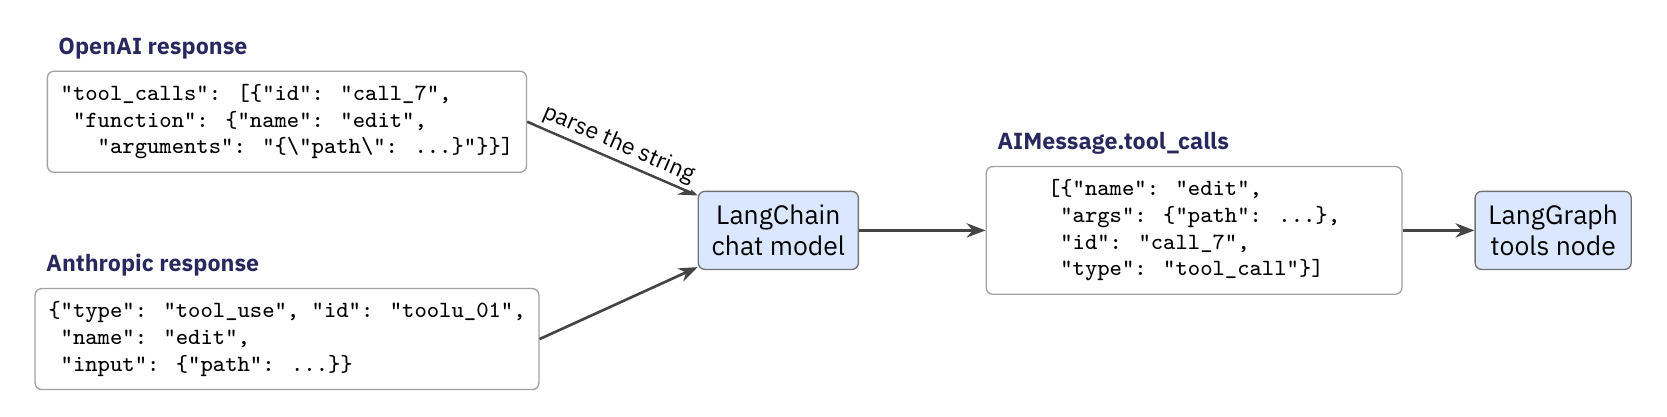
\includegraphics[width=0.92\textwidth]{figures/deck/3e51a79c67.png}
  \caption{LangChain's chat-model adapter converts an OpenAI reply and an Anthropic reply into
  one list, \texttt{AIMessage.tool\_calls}, which the tools node of the harness reads. The OpenAI
  arguments arrive as a string and are decoded on the way, and the Anthropic input arrives as an
  object and is copied.}
  \label{fig:native-adapters}
\end{figure*}

The native formats of OpenAI and Anthropic differ in their field names and agree in their
structure. Each has a tool definition in the request, a call with an identifier in the response,
and a result in the next request that repeats the identifier
\citep{openai-function-calling,anthropic-tooluse}. \Cref{tab:native-formats} sets the two formats
side by side. Each row names one part of the round trip, and its two cells give that part in each
vendor's format. The last row holds the one part that only Anthropic's format has.

The differences that matter to a harness are the following:
\bi
\item \textbf{Arguments.} OpenAI sends the arguments as a JSON string, which must be decoded before
the arguments can be bound. In \msa{}, LangChain's adapter decodes it (\cref{sec:native-adapters}).
Anthropic sends the arguments as a JSON object, which needs no decoding.
\item \textbf{Placement of results.} In OpenAI's format, the harness returns each result as a
message of its own, with the role \demoref{tool}. In Anthropic's format, the harness places the
results as \demoref{tool\_result} blocks inside a user message, and these blocks must come before
any text in that message.
\item \textbf{Errors.} Anthropic's result block has an optional flag, \demoref{is\_error}, that marks
a failed call. OpenAI's result message has no such field.
\ei

OpenAI's newer Responses API has the same parts under other names. A call is a
\demoref{function\_call} item with a \demoref{call\_id}, and its result is a
\demoref{function\_call\_output} item that repeats the \demoref{call\_id}.

\subsection{One list of calls for both formats}
\label{sec:native-adapters}

The harness of \msa{} never reads a vendor's format directly. It is built on LangGraph, a library
that runs an agent as a graph of nodes, and it calls the model through LangChain's chat-model
adapters, the classes through which LangChain calls each vendor's API. These adapters convert each
vendor's reply into one common message object, an
\demoref{AIMessage} \citep{langchain-messages}. Its attribute \demoref{tool\_calls} is a list with
one entry per call, and each entry holds the call's name, its arguments as a dictionary
(\demoref{args}) and its identifier (\demoref{id}).

\Cref{fig:native-adapters} follows both replies into the one list. For OpenAI, the adapter
decodes the argument string into the dictionary. For Anthropic, it copies the input object, which is
already a dictionary. A call whose arguments cannot be decoded goes to a separate list,
\demoref{invalid\_tool\_calls}. This is the case of \cref{sec:native-ids} in which a call receives
no result.

LangGraph runs the graph, and its tools node reads only the list \demoref{tool\_calls}. The same
harness code therefore runs with either vendor, and none of the code written for the harness handles
a vendor's format.

The tools node turns the list into results with a short loop (\cref{lst:native-toolsnode}). The
first line reads the list from the last message in the state record, which stores the run's
variables (Lecture~3). That last message is the model's reply. For each call, the loop passes the
name and the arguments to the dispatcher, which returns an observation. It then builds one tool
message per call, which LangChain calls a \demoref{ToolMessage}. The message's content is the
observation's result, and its \demoref{tool\_call\_id} repeats the call's identifier.

\begin{lstlisting}[basicstyle=\ttfamily\footnotesize, caption={Illustrative code for the loop of the tools node, abbreviated. Each call goes to the dispatcher, and each observation returns to the model as one tool message keyed by the call's identifier.}, label=lst:native-toolsnode]
for call in state["messages"][-1].tool_calls:
    observation = dispatcher(
        {"name": call["name"], "args": call["args"]})
    replies.append(ToolMessage(
        content=observation.result,
        tool_call_id=call["id"],
        name=call["name"]))
\end{lstlisting}

The loop runs the calls one after another, in the order in which they appear in the reply. Each
call finishes before the next one begins, so the effects of the calls follow their order in the
reply. If one reply asks for two edits of the same file, the second edit sees the file as the first
one left it.

\subsection{Guarantees of in-process tools}
\label{sec:native-local}

A tool that runs inside the harness's own process gives each call the guarantees of a local call,
as long as the harness runs one call at a time. We call such a tool an \textbf{in-process tool}. The
tools of \msa{}, \demoref{read\_file}, \demoref{search} and \demoref{edit}, are in-process tools. A
local call, as defined in \cref{sec:toolcalls}, is a call to a procedure in the caller's own
process.

Such a call has the following properties. The grouping is the course's own, and no single source
lists the properties together.
\bi
\item \textbf{A returned call shows that the tool ran.} When the tool function returns, the
dispatcher holds its result. When the function fails, the dispatcher holds the exception it raised.
Every call that reaches the tool function ends in one of these two outcomes, unless the tool hangs,
and the harness knows which one.
\item \textbf{One call runs the tool once.} No retry and no duplicate delivery sit between the
dispatcher and the tool. The retried request of \cref{sec:toolcalls}, which applied the same patch
twice, cannot occur inside one process.
\item \textbf{The harness and the tool fail together.} The tool is a function in the harness's
process. If the process crashes, both stop, so neither can keep running after the other has failed.
\item \textbf{No timeout is needed.} A tool that hangs also hangs the harness. The harness therefore
never has to guess whether a slow call has failed.
\item \textbf{Partial effects are visible.} A \textbf{partial effect} is a change that an operation
made before it failed. The tool and the harness share the files of the workspace, so the harness can
inspect what a failed tool changed and repair it.
\item \textbf{Effects happen in program order.} \textbf{Program order} means that effects occur in
the order of the calls in the reply. The tools node runs the calls of a reply one after another
(\cref{sec:native-adapters}).
\ei

No timeout is needed because a local caller never has to tell a slow callee from a dead one. Across
a boundary, a reply that has not arrived may mean that the callee is slow, that it has crashed, or
that the reply was lost (\cref{sec:toolcalls}). The caller must then choose how long to wait before
it gives up. A local call can still hang. A tool function that never returns blocks the whole
harness, and \cref{sec:codeact} returns to this problem, because one code action can hold any amount
of computation.

These guarantees come from where the tool runs and from how the harness runs it. The native format
contributes none of them, so prompted calling with an in-process tool has the same properties. They
hold only under the following conditions:
\bi
\item \textbf{The tool runs inside the harness.} A tool in another process, such as a tool that an
MCP server offers (\cref{sec:toolcalls}), receives each call as a message, and a message can be lost,
delayed or delivered twice.
\item \textbf{The harness runs one call at a time.} Parallel tool calls let a model place several
calls in one reply. A harness that ran them concurrently would lose program order.
\ei

Each of these properties can fail when a call crosses to another machine, because a remote call
differs from a local one in the ways that \cref{sec:toolcalls-rpc} listed, partial failure among
them \citep{waldo1994note}. Remote procedure calls kept the semantics of a local call where they could and
gave communication failures semantics of their own \citep{birrell1984rpc}. Results from distributed
computing explain why several of these properties are lost across a boundary:
\bi
\item \textbf{Ordering (program order).} Within one process, events are ordered by the sequence in which the process
executes them. Events in different processes can be ordered only through the messages between them
\citep{lamport1978time}. Inside the harness, the sequence of the calls alone therefore fixes their
order.
\item \textbf{Agreement (a returned call shows that the tool ran).} Two parties that communicate over a channel that can lose messages can
never both be certain of an outcome, a result known as the Two Generals problem
\citep{akkoyunlu1975constraints,gray1978notes}. A local call involves no such channel.
\item \textbf{Failure classes (failing together, no timeout needed).} A server can fail by omitting a reply, by replying too early or too
late, by replying with a wrong value, by crashing, or in arbitrary ways
\citep{cristian1991understanding}. A remote caller must allow for each of these failures.
\item \textbf{Repair (partial effects are visible).} An effect that has already been made permanent cannot simply be cancelled. A
later step, called compensation, must undo it \citep{garciamolina1987sagas}. An in-process tool lets
the harness inspect and repair the files directly.
\ei

\subsection{Requiring or forbidding tool calls}
\label{sec:native-choice}

\begin{table}[t]
  \caption{Request parameters with which an application controls tool calls in OpenAI's Chat
  Completions API and Anthropic's Messages API.}
  \label{tab:native-controls}
  \begin{adjustbox}{width=\linewidth}\begin{tabularx}{\linewidth}{L{0.24\linewidth}XX}
    \toprule
    \textbf{Control} & \textbf{OpenAI} & \textbf{Anthropic} \\
    \midrule
    \textbf{Require a call} & \demoref{tool\_choice} set to \demoref{"required"} or to a named
    function & \demoref{tool\_choice} of type \demoref{any} or \demoref{tool}, rejected by several
    of the newest Claude models and by any model on which extended thinking is turned on manually \\ \addlinespace[3pt]
    \textbf{Forbid calls} & \demoref{tool\_choice} set to \demoref{"none"} &
    \demoref{tool\_choice} of type \demoref{none} \\ \addlinespace[3pt]
    \textbf{At most one call per reply} & \demoref{parallel\_tool\_\allowbreak calls} set to false
    & \demoref{disable\_parallel\_\allowbreak tool\_use} set to true \\ \addlinespace[3pt]
    \textbf{Schema-valid arguments} & \demoref{"strict":\ true} in the tool definition &
    \demoref{"strict":\ true} in the tool definition \\
    \bottomrule
  \end{tabularx}\end{adjustbox}
\end{table}

The application can tell the model API whether a reply must contain a tool call, may contain one,
or must contain none. The request parameter that does this is called \textbf{tool choice}: it
requires, allows or forbids tool calls. Requiring a call is called \textbf{forced tool use}, and it
demands a call to some tool or to a named tool. \Cref{tab:native-controls} lists the parameters of
both vendors, together with the controls of \cref{sec:native-arguments}.

Both vendors accept the setting \demoref{auto}, which lets the model decide, and the setting
\demoref{none}, which forbids calls. OpenAI's Chat Completions API requires a call with
\demoref{required}, or with a named function when one particular tool must be called
\citep{openai-function-calling}. Anthropic's API requires a call with \demoref{any}, which demands
some tool, or with \demoref{tool}, which demands a named tool \citep{anthropic-define-tools}.

Requiring a call suits a task that must always produce structured output, such as extracting the
fields of an invoice. The application defines a tool whose arguments are those fields, for example
one named \demoref{record\_invoice}. With OpenAI, it forces a call to that tool. Every reply then
contains the call, and the call's arguments are the extracted fields in the shape that the argument
schema fixes.

Anthropic restricts forcing. Several of the newest Claude models reject forced tool use whatever
their settings. So does any Claude model on which the application has turned on extended thinking
manually, a setting in which the model reasons at length before it replies.

On these models, the alternative is \demoref{auto} together with strict mode, which Anthropic calls
strict tool use, or structured outputs, a feature that makes the whole reply follow a fixed JSON
schema. With \demoref{auto}, the model may still answer without calling the tool. Strict mode then
guarantees only that the arguments are valid whenever the model does call it.

Forbidding calls works with both vendors and with every Claude model, and it suits the end of a
budgeted run. In Lecture~3's budgeted loop, a run may make only a fixed number of model calls, 40 in
\msa{}. The harness can make the last call that the budget allows with tool choice set to
\demoref{none}. The model then cannot request another tool, so the run ends with a text answer.
Without this setting, the model could request a tool on that last call, and the tool's result would
never reach the model.

\subsection{Limiting calls and their arguments}
\label{sec:native-arguments}

% A figure* floats to the top of a later page, so it is placed here to appear beside
% \cref{sec:native-limits}, which uses it.
\begin{figure*}[t]
  \centering
  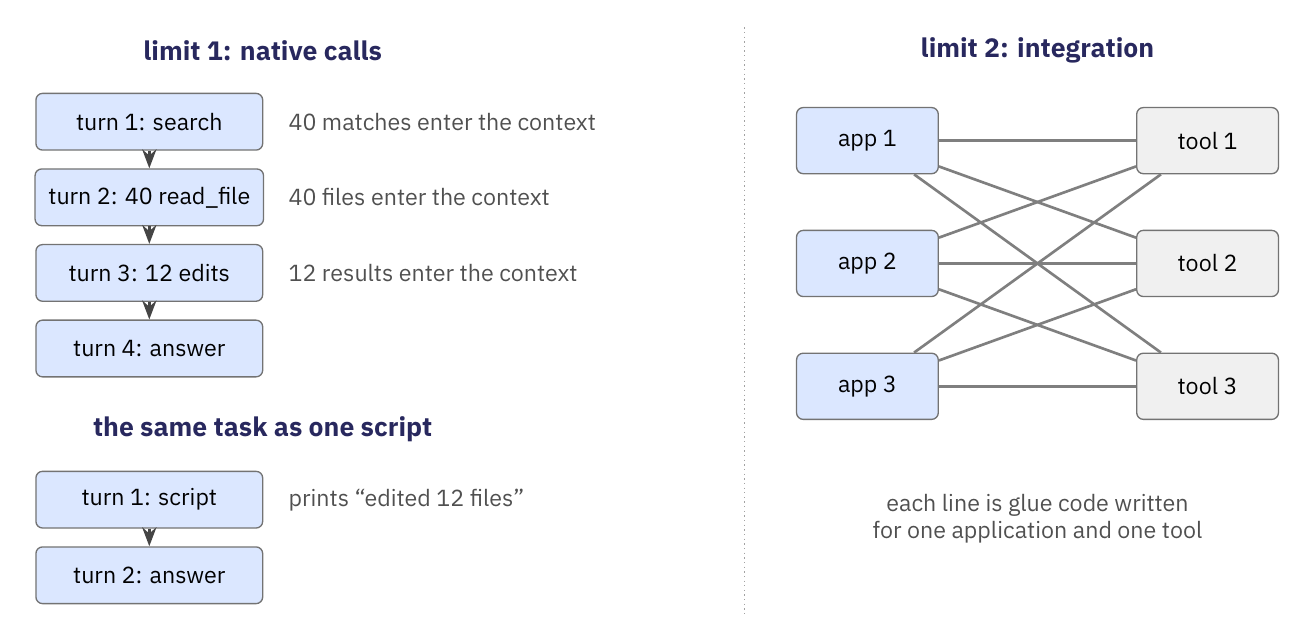
\includegraphics[width=0.78\textwidth]{figures/deck/6eec671dd0.png}
  \caption{Left: a task that edits only the files in which a search match lies inside a loop of the
  source code, done with native calls and done as one script, with illustrative numbers. Right:
  three applications and three tools, where each line is integration code written for one
  application and one tool.}
  \label{fig:native-limits}
\end{figure*}

Further request parameters limit how many calls a reply may hold and which arguments a call may
carry. Disabling parallel tool calls limits each reply to at most one call. OpenAI does this with the
parameter \demoref{parallel\_tool\_calls} set to false. Anthropic does it with the field
\demoref{disable\_parallel\_tool\_use} set to true inside the tool choice \citep{anthropic-tooluse}.

One call per reply serves edits that depend on one another and must run in order. Each edit then
runs, and its result returns, before the model asks for the next one. Program order then no longer
depends on how the harness runs the calls of a reply, because no reply holds more than one call.
The cost is extra turns. A turn is one pass through the loop, from one model call to the next
(Lecture~2), and work that a single reply could have requested now takes one turn per tool call.

Strict mode guarantees that the arguments of a call match the tool's argument schema. Without it, a
call may carry an argument of the wrong type, for example \demoref{\{"path":\ 7, ...\}} where the
schema requires the path to be a string. Both vendors offer strict mode as a flag,
\demoref{"strict":\ true}, on the tool definition, and both implement it by constrained decoding
\citep{openai-function-calling,anthropic-strict-tool-use}.

In \textbf{constrained decoding}, at each step of generation, the model may choose only tokens that
keep the output valid under the schema \citep{openai2024structuredoutputs}. A model normally samples
each token from its whole vocabulary. Under constrained decoding, every token that would break the
schema is excluded, so arguments that the model finishes decode and match the schema. The
guarantee does not cover a reply that is cut off early, for example at the reply's length limit, or
a reply in which the model refuses the request. Anthropic also documents that strict mode does not
guarantee capitalization when the schema restricts a string to a fixed list of values, an enum. A
returned value can then differ from a listed value in its capital letters
\citep{anthropic-structured-outputs}.

The guarantee holds only within the subset of JSON Schema that strict mode supports, and a request
whose schema leaves that subset is rejected. OpenAI's strict mode, for example, requires
\demoref{"additionalProperties":\ false}, which forbids fields that the schema does not list, and it
requires every property to be listed as required. Anthropic's strict mode accepts properties that
are not required.

Each vendor thus accepts a different subset, so the subset becomes part of the tool's contract. The
argument schema must be written within it, and a tool moved to another vendor may need its schema
rewritten.

The guarantee also covers only the shape of the arguments (\cref{sec:toolcalls}). A call whose path
is a string, as the schema demands, can still name the wrong file.

\subsection{Limits of native tool calling}
\label{sec:native-limits}

Native tool calling is limited in what one reply can express and in how a tool reaches the applications
that use it. The first limit is that a reply cannot loop or branch. A reply is a list of calls that
the model fixes when it writes the reply. It cannot say ``for every match, read the file'', and it
cannot say ``if the match lies inside a loop of the code, edit the file''.

Every decision that depends on a result therefore costs a turn. Every result also enters the model
context, what one model call receives (Lecture~3).

\Cref{fig:native-limits} shows both limits. Its left side counts the turns of one task done with
native calls and done as one script, and its right side draws the integration code between three
applications and three tools. The task edits only the files in which a search match lies inside a
\texttt{for} or \texttt{while} loop of the source code.

With native calls, the first turn searches, and all the matches enter the model context. The second turn
reads every matching file, and every file enters the model context. Parallel tool calls let the model
batch these reads into one reply, but the choice of the files to edit still waits for the next turn.
The third turn edits the files that qualify, and the fourth turn answers.

Suppose instead that the model could write a script, a short program that the harness runs
(\cref{sec:codeact}). The script makes the same decisions within one turn and prints only a summary,
such as the number of files it edited. Every result that passes through the model context costs tokens and
time. The script keeps those results out of the model context and needs fewer turns.

The second limit is that each application integrates each tool itself, in its own language and in
its vendor's format. Every pair of an application and a tool needs its own integration code, so
three applications and three tools need nine pieces of it.

Code actions address the first limit: the model writes a program, which can loop and branch over
results within one turn (\cref{sec:codeact}). The Model Context Protocol addresses the second: a
server offers its tools once, through one protocol, and any application that speaks the protocol can
list and call them. Lecture~5 studies the protocol, and the end of \cref{sec:codeact} returns to the
integration problem.

\subsection*{Key points}
\bi
\item A tool call is native when the model API defines its format: the request carries the tool
definitions, the reply returns each call in a structured field, and the provider builds the prompt
from the definitions and parses the model's output.
\item Every native call carries a call identifier that its result must repeat, and the harness of
\msa{}, which alone decides whether a call runs, returns a tool message for every call it receives,
refused calls included.
\item OpenAI's and Anthropic's formats differ in field names and share a tool definition, a call with
an identifier and a result that repeats it, and LangChain converts both into the one list that the
tools node reads.
\item An in-process tool that the harness runs one call at a time gives each call the guarantees of
a local call, whether the call is native or prompted: a returned call shows that the tool ran, one
call runs the tool once, harness and tool fail together, no timeout is needed, partial effects are
visible, and effects follow program order.
\item Tool choice requires, allows or forbids tool calls, and disabling parallel tool calls keeps
program order at the cost of extra turns.
\item Strict mode uses constrained decoding to make the arguments match the argument schema, within
the subset that the vendor supports, and a call that matches the schema can still name the wrong
file.
\item A native reply cannot loop or branch, which code actions address, and each application must
integrate each tool itself, which the Model Context Protocol addresses.
\ei

\section{Code actions}
\label{sec:codeact}

Native tool calls have a limit that \cref{sec:native} identified. A reply cannot loop or branch, so
every decision that depends on a tool result costs a turn, and every result passes through
the model context. Code actions remove this limit by making the model's action a program, which
the harness runs in an interpreter. The harness then no longer sees the individual operations, so
the dispatcher's checks and its per-call records no longer apply, and the budget on model calls no
longer bounds the work of a single action. This section shows what a design based on code actions
needs instead: a sandbox that confines writes, a record of each program's effects, limits that bound
its work, and care with instructions that arrive in observations. It ends with the second limit of
native calls, the cost of integrating every tool into every application separately, which leads to
Lecture~5.

\subsection{Code as the action}
\label{sec:codeact-action}

A \textbf{code action} is an action written as a program that the harness runs in an interpreter.
\textbf{CodeAct} is the approach in which the model's action is Python code, so that loops and
conditions run inside a single turn \citep{wang2024codeact}. With native calls, the model requests
one operation per call, and the dispatcher executes each call (\cref{sec:dispatcher}). With
CodeAct, the model writes the operations, and the control flow between them, as one program.

\Cref{lst:codeact-actions} shows the difference on an illustrative task: replace the comparison
\texttt{i <= n} with \texttt{i < n} in every Python file under \texttt{src}. The first action is a
\textbf{JSON action}, a tool call written as a JSON object that names the tool and its arguments.
It calls the \demoref{edit} tool of \msa{} once and changes one file. A native tool call is one kind
of JSON action. In the CodeAct study of \cref{sec:codeact-evidence}, JSON actions were written as
text in a format that the prompt described. The second action is a code action.
It loops over every Python file under \texttt{src} and rewrites each one. With JSON actions, the
same change needs one call per file, and further calls to find the files first, because a single
call cannot loop or branch.

\begin{lstlisting}[float=tbp, basicstyle=\ttfamily\footnotesize, columns=fixed, basewidth=0.525em, caption={Illustrative actions for the task of replacing \texttt{i <= n} with \texttt{i < n}. Above, a JSON action that edits one file. Below, a code action, sent as a shell command, that edits every matching file.}, label=lst:codeact-actions]
{"name": "edit",
 "arguments": {"path": "src/parse.py",
               "old": "i <= n", "new": "i < n"}}

python - <<'EOF'
import pathlib, re
for f in pathlib.Path("src").rglob("*.py"):
    s = f.read_text()
    f.write_text(re.sub(r"i <= n", "i < n", s))
EOF
\end{lstlisting}

The code action is a shell command. Its first line is shell syntax that passes the following
lines, up to \texttt{EOF}, to the Python interpreter as its input. A coding agent often sends its
code in this form, through a tool that runs shell commands. The Python interpreter of CodeAct
(\cref{sec:codeact-loop}) instead receives the Python lines directly. Both forms are code actions.
As in \cref{sec:native}, we call the program that a code action carries a script.

Inside the script, \texttt{rglob("*.py")} finds every Python file under \texttt{src} at any depth.
\texttt{re.sub} replaces every occurrence of the pattern, and \texttt{write\_text} saves the file.

The script never calls \demoref{edit}. It reads and writes the files with ordinary Python, so none
of the dispatcher's checks applies. No registry lookup or binding takes place. The path check
inside \demoref{edit} never runs, and neither does \demoref{edit}'s rule that \texttt{old} must
occur exactly once: \texttt{re.sub} replaces every occurrence. The trace records no
\demoref{tool\_request} or \demoref{tool\_result} event for any of the writes.

With code actions, the interpreter takes the place of the argument schema as the limit on what an
action may do. With native calls, the tool contract (\cref{sec:toolcalls}) states which arguments a
call may carry, and the harness checks each call against it before the tool runs. An interpreter
accepts any program it can parse. Validating arguments becomes validating code, which is much
harder, because what a program does can depend on values it computes while it runs
(\cref{sec:codeact-sandbox}).

The interpreter therefore needs a \textbf{sandbox}, an environment in which the operating system
confines a process, so that the process can reach only the resources that the environment grants.
A \textbf{container} is a common kind of sandbox: the operating system runs the process with its
own view of the files, the network and the other processes. The difficult problems in a design
based on code actions are validating code and building this sandbox.

\subsection{Evidence for code actions}
\label{sec:codeact-evidence}

In a study of 17 language models, code actions were comparable to actions written as JSON or text,
or better, on single tool calls for most models. On tasks that combine several tools, code actions
were the best format for 12 of the 17 models \citep{wang2024codeact}. The CodeAct study compared
three action formats: Python code, JSON, and text in a format that the prompt describes. It used
two benchmarks:
\bi
\item \textbf{Single calls.} On API-Bank, each task needs one call to one tool, so the loops and
conditions of a program bring no advantage. The study measured whether each call was correct.
CodeAct was comparable to the other formats or better for most models, and it was the best format
for 8 of the 17.
\item \textbf{Several tools over several turns.} M3ToolEval, the study's own benchmark, has 82
tasks that typically need several calls to several tools over several turns. The study measured
the success rate and the average number of turns. CodeAct was the best of the three formats, ties
included, for 12 of the 17 models. For the model with the highest success rate overall, CodeAct's
success rate was 20.7 percentage points higher than that of the next-best format. CodeAct also
needed the fewest turns on average for 12 of the 17 models.
\ei

The study does not show that code actions beat every alternative. The baselines were formats
described in the prompt, that is, prompted calling (\cref{sec:toolcalls}). Native tool calling was
not among them, so the study does not compare code actions with native calls. The largest gains
appeared on the authors' own benchmark of multi-tool tasks, and on neither benchmark was CodeAct
the best format for every model. The study measured the correctness of calls, the success rate of
tasks and the number of turns. It did not measure the cost of running model-written code safely,
which is the subject of the rest of this section.

\subsection{How a code action runs}
\label{sec:codeact-loop}

In CodeAct, the harness runs each script the model sends in a Python interpreter and returns the
script's output to the model as the next observation. The interpreter is a \textbf{kernel}: a
persistent Python process that runs each script and keeps its variables between turns, as a
Jupyter kernel does. Connected to such an interpreter, the model can revise earlier actions or
issue new ones as new observations arrive over several turns \citep{wang2024codeact}.

\begin{figure*}[t]
  \centering
  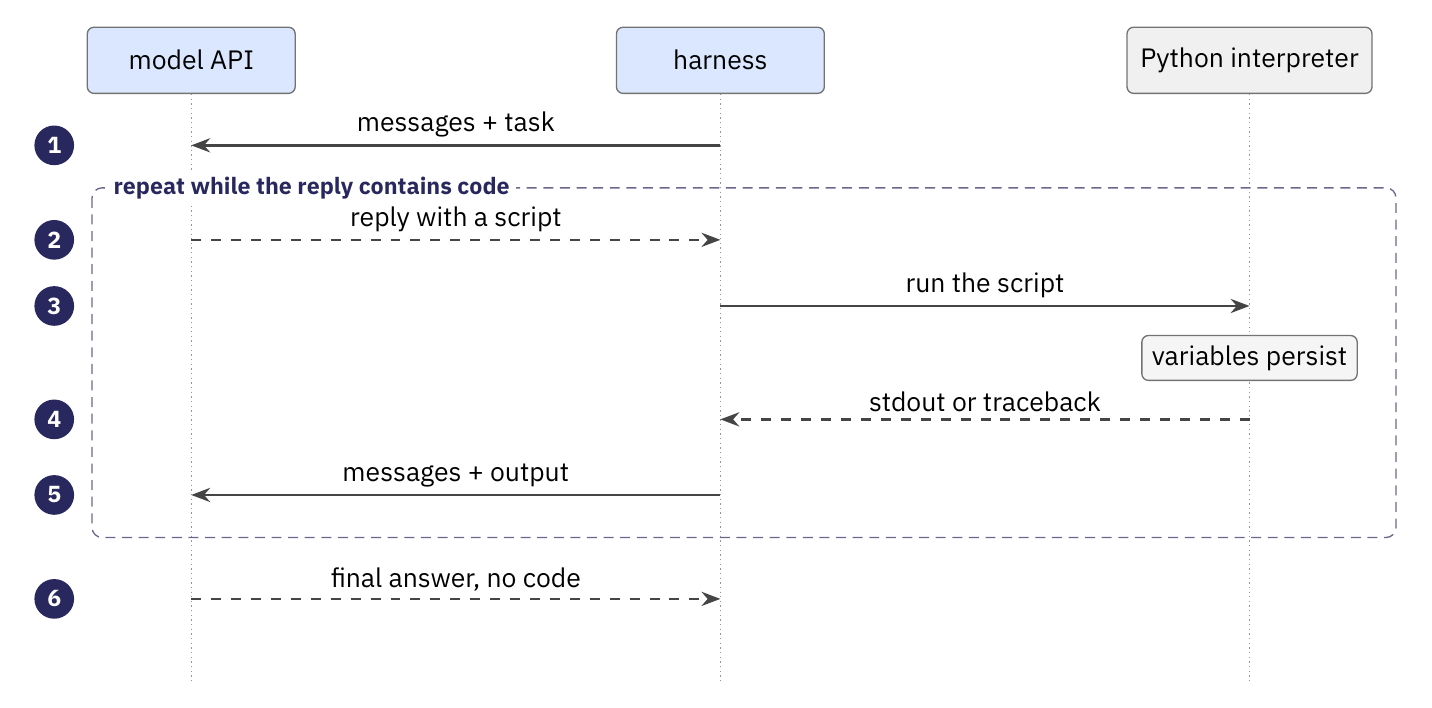
\includegraphics[width=0.72\textwidth]{figures/deck/5a0af0876d.png}
  \caption{One CodeAct run. The harness passes each script from the model to the Python
  interpreter (the kernel) and returns the output as the next observation, until a reply contains
  no code.}
  \label{fig:codeact-loop}
\end{figure*}

\Cref{fig:codeact-loop} follows one run. Its numbered steps are the following:
\be
\item The harness sends the messages, including the task, to the model.
\item The model replies with a script.
\item The harness runs the script in the kernel. Variables that the script defines stay in the
kernel for later scripts.
\item The kernel returns what the script printed or, if the script raised an exception, the
\textbf{traceback}, Python's report of the error and of the calls that led to it.
\item The harness appends this output to the messages as the next observation and calls the model
again.
\item When a reply contains no code, the harness treats it as the final answer and ends the run.
\ee
Steps 2 to 5 repeat as long as the model's replies contain code.

There are no tool calls in this loop. The script reads and writes files, imports packages and
starts processes with ordinary Python. This lets the model use existing software packages in place
of tools written by hand for the task. It also means that a single reply carries a whole program,
which may contain any number of operations, where a native call carries one.

\subsection{A minimal kernel}
\label{sec:codeact-kernel}

A kernel for CodeAct needs only a few lines of Python, because the interpreter does the work of
running the action. \Cref{lst:codeact-kernel} is a minimal kernel written for the lecture. It is
the whole execution side of CodeAct: it has no tool functions, no registry and no dispatcher. The
numbered comments mark the lines explained below.

\begin{lstlisting}[basicstyle=\ttfamily\footnotesize, columns=fixed, basewidth=0.525em, caption={Illustrative minimal kernel. It extracts the script from the model's reply, runs it in one namespace, and returns the output or the traceback.}, label=lst:codeact-kernel]
import io, re, traceback
from contextlib import redirect_stdout

namespace = {}                             # 1

def extract(reply: str) -> str | None:
    m = re.search(r"```python\n(.*?)```",
                  reply, re.S)             # 2
    return m.group(1) if m else None

def run(script: str) -> str:
    out = io.StringIO()
    try:
        with redirect_stdout(out):
            exec(script, namespace)        # 3
    except Exception:
        out.write(traceback.format_exc())  # 4
    return out.getvalue()                  # 5
\end{lstlisting}

\bi
\item \textbf{The namespace (1).} A \textbf{namespace} is the dictionary of names, such as
variables, functions and imported modules, in which the scripts run. It starts empty. When the
first script runs, Python inserts one entry, \texttt{\_\_builtins\_\_}, through which the script
reaches the built-in functions, such as \texttt{print}, \texttt{open} and \texttt{\_\_import\_\_}.
\item \textbf{The script (2).} The harness takes the script from the fenced Python block of the
model's reply, the text between
\texttt{\textasciigrave\textasciigrave\textasciigrave python} and the closing fence. A reply
without such a block yields no script, which is the signal that ends the run.
\item \textbf{Execution (3).} The built-in function \texttt{exec} runs the script in the
namespace. The script runs with every right of the harness process: it can read and write every
file the harness can, open network connections and start other programs.
\item \textbf{Errors (4).} An error in the script, such as a \texttt{NameError}, does not stop the
harness. The kernel catches it and writes the traceback into the output.
\item \textbf{The observation (5).} Everything the script printed, followed by any traceback, is
returned and becomes the next observation.
\ei

The same namespace serves every turn, so variables persist between scripts. A variable that one
script defines, such as a list of matching files, is available to the next script without being
computed again.

Some frameworks, such as smolagents, also place selected functions in the namespace, so that a
script can call tools as ordinary Python functions (\cref{sec:codeact-frameworks}). This is a
variant of the design. What defines CodeAct is that the action is a program, whether or not the
namespace holds tools.

\subsection{A run in the kernel}
\label{sec:codeact-run}

A CodeAct run alternates scripts and their outputs, and the model can correct a failed script from
its traceback. \Cref{lst:codeact-run} is a constructed transcript, written for the lecture with the
kernel above. It is not a recorded run. Each observation is the output of \texttt{run} for one
script, sent to the model as a user message.

\begin{lstlisting}[basicstyle=\ttfamily\footnotesize, columns=fixed, basewidth=0.525em, caption={Constructed CodeAct transcript for the task of \cref{lst:codeact-actions}. The scripts are shown without the fences that enclose them in the replies.}, label=lst:codeact-run]
system    Solve the task by writing Python in a
          ```python block. Print what you need.
user      Replace i <= n with i < n in every
          file under src.
assistant import pathlib
          hits = [p for p in
                  pathlib.Path("src").rglob("*.py")
                  if "i <= n" in p.read_text()]
          print(hits)
user      Observation: [PosixPath('src/parse.py'),
                        PosixPath('src/scan.py')]
assistant for p in hits:
              p.write_text(re.sub("i <= n", "i < n",
                                  p.read_text()))
user      Observation: Traceback (most recent call
          last): ...
          NameError: name 're' is not defined
assistant import re
          for p in hits:
              p.write_text(re.sub("i <= n", "i < n",
                                  p.read_text()))
              print("edited", p)
user      Observation: edited src/parse.py
                       edited src/scan.py
assistant Both comparisons under src now read i < n.
\end{lstlisting}

The model's replies proceed as follows:
\bi
\item \textbf{The first script} only gathers information. It lists the Python files under
\texttt{src} that contain the comparison, stores them in the variable \texttt{hits}, and prints the
list.
\item \textbf{The second script} uses \texttt{hits} without computing it again, because both
scripts run in the same namespace. It fails with a \texttt{NameError} because no script has
imported the module \texttt{re}. The kernel's own import of \texttt{re} in \cref{lst:codeact-kernel}
does not help, because a script sees only the names in its namespace, and the kernel's imports are
not among them. Python evaluates \texttt{re.sub} before it calls \texttt{write\_text}, so the script
fails before its first write, and the files are unchanged.
\item \textbf{The third script} adds the missing import, which the model found from the traceback,
and repeats the writes, printing each file it changed. Correcting code from the error message that
running it produced is called \textbf{self-debugging}, and it is one of the benefits of code
actions \citep{wang2024codeact}.
\item \textbf{The final reply} contains no code, so \texttt{extract} finds no script and the harness
ends the run.
\ei

The harness saw three scripts and their outputs. It saw none of the individual file reads and
writes, because these happened inside the interpreter. With native calls, each edit would have
passed through the dispatcher and left a request and a result in the trace
(\cref{sec:dispatcher}). In this run, the only report of what the third script changed is what the
script chose to print. \Cref{sec:codeact-diff} returns to this loss of visibility.

\subsection{Code actions in agent frameworks}
\label{sec:codeact-frameworks}

Code actions are used in agent frameworks and in published designs, which differ in how the model
writes its code and in where that code runs. \Cref{tab:codeact-frameworks} compares smolagents,
OpenHands and Anthropic's code execution with MCP on these two points.

\begin{table*}[t]
  \caption{Code actions in smolagents, OpenHands and Anthropic's code execution with MCP: how the
  model acts and where its code runs.}
  \label{tab:codeact-frameworks}
  \begin{adjustbox}{width=\linewidth}\begin{tabularx}{\linewidth}{L{0.24\linewidth}XX}
    \toprule
    \textbf{System} & \textbf{How the model acts} & \textbf{Where the code runs} \\
    \midrule
    \textbf{smolagents CodeAgent} & The model writes Python snippets that call tools, which the
    framework provides as Python functions. & A local executor that allows only listed imports,
    or a remote sandbox such as E2B, Docker, Modal or Blaxel. \\
    \textbf{OpenHands CodeActAgent} & The model acts through bash commands and Python code,
    following the CodeAct approach. & By default, a Docker container that the platform manages.
    Local and remote execution environments also exist. \\
    \textbf{Code execution with MCP (Anthropic)} & A design proposal. The model writes TypeScript
    against tools from external MCP servers, which appear to it as files. & A sandboxed execution
    environment that the design proposes. Intermediate results stay there, outside the model
    context. \\
    \bottomrule
  \end{tabularx}\end{adjustbox}
\end{table*}

Each row raises a point about safety or evidence:
\bi
\item \textbf{smolagents.} Its local executor does not pass the script to \texttt{exec}. It reads
the script's syntax tree, the structure that Python builds when it parses code, runs it operation
by operation and allows only listed imports. Its documentation nevertheless states that no local
Python sandbox can be completely secure, and it recommends remote executors for code that needs
strong isolation \citep{smolagents-secure-execution}. These restrictions reduce the risk of the
local executor without removing it.
\item \textbf{OpenHands.} Its CodeActAgent, which the documentation now archives as a legacy agent,
implements the CodeAct idea, and by default its code runs in a Docker container
\citep{openhands-docs}. The container places a boundary that the operating system enforces around
every script, the measure that \cref{sec:codeact-sandbox} shows to be necessary.
\item \textbf{Code execution with MCP.} This is a design proposal in an Anthropic engineering post
\citep{jones2025codeexecmcp}. It describes no deployed agent. The tools come from servers
outside the application through MCP (\cref{sec:toolcalls}). The model finds them as files, loads
only the definitions it needs, and keeps intermediate results in the execution environment. For
one example, the post estimates that token usage falls from 150,000 to 2,000, a reduction of
98.7\%. This number illustrates one example. It is not a measurement over many tasks.
\ei
Cloudflare describes the same design as Anthropic's post under the name Code Mode. In Code Mode, the
model writes code that calls its tools instead of calling them one at a time, and the tools are
presented to it as a TypeScript API \citep{varda2025codemode}.

Running agent-generated code safely requires a secure execution environment with sandboxing,
resource limits and monitoring. Each requirement answers a problem that code actions create, and
the following subsections take these problems one at a time as worked questions. Sandboxing
confines the writes of a script (\cref{sec:codeact-sandbox}). Monitoring records what each script
changed (\cref{sec:codeact-diff}), and staging lets the harness withhold those changes
(\cref{sec:codeact-staging}). Resource limits bound the work of a script
(\cref{sec:codeact-limits}). Instructions that arrive in observations are a further problem, which
none of these measures prevents (\cref{sec:codeact-injection}).

\subsection{Confining writes: the sandbox}
\label{sec:codeact-sandbox}

Only a check that the operating system makes, outside the Python interpreter, can confine every
file access of a script.
Consider a model that sends the script of \cref{lst:codeact-escape-write}, which writes a file in
the parent directory of the workspace.

\begin{lstlisting}[basicstyle=\ttfamily\footnotesize, columns=fixed, basewidth=0.525em, caption={Illustrative script that writes outside the workspace.}, label=lst:codeact-escape-write]
import pathlib
pathlib.Path("../config.yaml").write_text("debug: true")
\end{lstlisting}

Which component can stop this script from writing outside the workspace? The operating system can,
provided that the interpreter runs in a sandbox in which the workspace is the only directory of the
host machine that the script can reach. The other plausible components fail:
\bi
\item \textbf{The prompt.} An instruction to stay inside the workspace describes the rule. Nothing
enforces it, so the model may still write a script that breaks it.
\item \textbf{A scan of the script's text.} The harness could search the script for paths before it
calls \texttt{exec}. Such a scan compares the text with a \textbf{blocklist}, a list of forbidden
patterns. The same
path can be built while the script runs, with string operations, \texttt{os.path.join} or a
variable, so no scan of the text finds every spelling.
\item \textbf{The dispatcher and the path check.} CodeAct has no dispatcher, and the script never
calls \demoref{edit}, so the path check inside it never runs. The harness hands one script to
\texttt{exec} and sees no individual calls, so there is nothing to check call by call.
\ei

The operating system succeeds where these fail because every file access of a script, however its
path was spelled, reaches the operating system as a request that it checks against what the
process may access. A check at that level therefore applies to every access.

A suitable sandbox for the kernel is a container (\cref{sec:codeact-action}) with no network and a
read-only root filesystem, that is, the container's own system files, which no script can change.
The container mounts one directory read-write, the workspace. Mounting a directory of the host
machine makes it appear at a path inside the container.

In such a container, the directory above the workspace on the host machine does not exist for the
script. The path \texttt{../config.yaml} resolves to a location in the container's read-only root,
so the write fails, however the script spells the path. This is complete mediation
(\cref{sec:dispatcher}) moved from the path check inside the tools to the sandbox. Every request for a protected
resource still passes through a guard, and with code actions the guard is the operating system.

Removing Python's built-ins from the namespace is only a partial measure. A namespace that holds
only \texttt{print} and \texttt{len} (the first line of \cref{lst:codeact-escape}) blocks
\texttt{open} and \texttt{import}, because the script can no longer name them.

\begin{lstlisting}[basicstyle=\ttfamily\footnotesize, columns=fixed, basewidth=0.525em, caption={Illustrative namespace without built-ins (first line) and a known way around it that needs no built-in (second line).}, label=lst:codeact-escape]
namespace = {"__builtins__": {"print": print, "len": len}}
().__class__.__base__.__subclasses__()
\end{lstlisting}

Every Python object still leads to its class, and every class leads to \texttt{object}, so a script
can reach other classes without naming any built-in. The second line starts from an empty
tuple, moves to its class and then to \texttt{object}, the base class of all Python classes, and
lists the classes that inherit directly from \texttt{object}. These are a large share of the
classes loaded in the process. Some of them lead to modules with functions that open files or
start processes, so a script can reach those functions without any built-in. A restricted
namespace therefore cannot replace the container.

\subsection{Recording effects: the workspace diff}
\label{sec:codeact-diff}

With code actions, the harness can record each script's effect on the files. The operations that
produced the effect stay hidden inside the interpreter. Consider a script that rewrites the
comparison in every Python file under \texttt{src} (\cref{lst:codeact-loop-fail}).

\begin{lstlisting}[basicstyle=\ttfamily\footnotesize, columns=fixed, basewidth=0.525em, caption={Illustrative script whose loop fails partway.}, label=lst:codeact-loop-fail]
import pathlib, re
for p in pathlib.Path("src").rglob("*.py"):
    p.write_text(re.sub("i <= n", "i < n",
                        p.read_text()))
\end{lstlisting}

The order in which \texttt{rglob} returns the files is not guaranteed, so we fix one for the
example. The loop rewrites \texttt{src/parse.py} first. The write to the next file,
\texttt{src/lexer.py}, then fails because that file is read-only, and \texttt{src/scan.py} is never
reached. What does the harness record for the turn? It records one script and its traceback, and
\texttt{src/parse.py} remains changed. The other plausible answers fail:
\bi
\item \textbf{One event per file write.} The writes happen inside \texttt{exec}, where the harness
sees nothing, so there are no per-write events.
\item \textbf{No record, because the script raised an exception.} The kernel catches the exception
and returns the traceback as the output, so the turn is recorded like any other.
\item \textbf{The kernel restores the changed file.} Nothing in the kernel restores files, so the
first write stays in the workspace.
\ei

The trace therefore no longer shows which writes happened. The failure leaves a partial effect,
the changes that an operation made before it failed (\cref{sec:native}). The traceback shows which
write failed. The record does not show which files the script changed before the failure. With
tools called one at a time through the dispatcher, each write would have its own request and
result in the trace.

Because there are no calls to log, the harness records the effect instead. A snapshot of the
workspace maps the path of every file to a hash of its contents, a short fingerprint that differs,
in practice, whenever the contents differ. A \textbf{workspace diff} is the record of the files
that each script created, changed or deleted, computed from snapshots taken before and after the
script. Comparing the two snapshots gives the files that changed or appeared and the files that
disappeared. \Cref{lst:codeact-diff} computes a workspace diff, and the harness appends both lists
to the trace with the script and its output.

\begin{lstlisting}[basicstyle=\ttfamily\footnotesize, columns=fixed, basewidth=0.525em, caption={Illustrative recording of a workspace diff around each script. Imports and the definitions of \texttt{WORKSPACE} and \texttt{trace} are omitted.}, label=lst:codeact-diff]
def run_recorded(script: str) -> str:
    before = snapshot(WORKSPACE)
    output = run(script)
    after = snapshot(WORKSPACE)
    trace.append({"event": "script",
        "script": script, "output": output,
        "changed": sorted(p for p in after
                     if before.get(p) != after[p]),
        "deleted": sorted(set(before) - set(after))})
    return output

def snapshot(root: Path) -> dict:  # path -> hash
    return {str(p):
              hashlib.sha256(p.read_bytes()).hexdigest()
            for p in root.rglob("*") if p.is_file()}
\end{lstlisting}

For the failed loop, the workspace diff lists only \texttt{src/parse.py} as changed, so the trace
again shows the partial effect of the failed script. The diff shows
what changed. It does not show how the script changed it or in which order. The diff also covers
only the workspace, so it is a complete record of the script's file changes only when the sandbox
prevents writes anywhere else (\cref{sec:codeact-sandbox}). In production, the same record comes
from running \texttt{git status} and \texttt{git diff} after each script, or from a snapshot of the
filesystem.

\subsection{Staging a script's effects}
\label{sec:codeact-staging}

Staging keeps a failed script from leaving a partial effect in the workspace. \textbf{Staging}
means running a script in a copy of the workspace and copying the result back only if the script
finished without an exception. The harness creates a temporary directory, copies the workspace into
it, and runs the kernel with its working directory, or its container's mount, set to the copy. If
the script raised an exception, the harness returns the output with a note that no changes were
applied, and the workspace stays as it was before the turn. Otherwise, the harness copies the
staged result back into the workspace. For the failed loop of \cref{sec:codeact-diff}, staging
leaves \texttt{src/parse.py} unchanged.

A simple copy-back has gaps that production systems close. It does not remove files
that the script deleted, because copying the staged directory over the workspace adds and
overwrites files but deletes none. It is also not atomic. An \textbf{atomic} operation either
completes entirely or has no effect. A crash during the copy-back leaves a mixture of old and new
files. A git worktree (a second checkout of the same repository) or an overlay filesystem (which
keeps the changes in a separate layer above an unchanged base) also records the script's deletions,
so applying the result removes the deleted files. Applying the result atomically needs a step that
takes effect at once, such as a rename that puts the staged directory in the workspace's place.

Staging also makes a script's effect reviewable before it is applied. A person or an automated
check can inspect the staged copy, or its workspace diff, and decide whether to copy it back.

\subsection{Bounding a script: resource limits}
\label{sec:codeact-limits}

A budget on model calls cannot stop a script that never ends. Only limits enforced outside the
script can. Suppose the budget allows 40 model calls and the model sends the script of
\cref{lst:codeact-spin}, which waits for a file that nothing creates.

\begin{lstlisting}[basicstyle=\ttfamily\footnotesize, columns=fixed, basewidth=0.525em, caption={Illustrative script that never ends, because nothing creates the file it waits for.}, label=lst:codeact-spin]
import os
while not os.path.exists("build/done"): pass
\end{lstlisting}

What stops this script? Nothing in the kernel: \texttt{exec} runs until something outside it kills
the process. The other plausible answers fail:
\bi
\item \textbf{The budget.} Each model node checks the budget before it calls the model, which is
Lecture~3's admission check. An iteration of the loop is not a model call, and the script never
returns control to the model, so the budget is never checked again.
\item \textbf{The kernel's exception handler.} The \texttt{try} and \texttt{except} of the kernel
catch exceptions, and an endless loop raises none.
\item \textbf{The model.} The model is waiting for the observation, and it cannot act until the
script returns.
\ei

One code action can contain any amount of computation, so a bound on model calls no longer bounds
the work of a run. This breaks Lecture~3's termination argument. That argument uses a loop variant,
a nonnegative integer that decreases on every continuing cycle. A continuing cycle is one pass
around a loop of the graph after which the run does not end. In \msa{}, the variant is the number of model calls remaining in
the budget. Because it cannot fall below zero, it bounds the number of continuing cycles. The argument holds only if every step between two
model calls returns or times out, and a script that never returns violates this condition.

The remedy is to give each script resource limits. \textbf{Resource limits} are bounds on a
script's CPU time, its memory, its wall-clock time and the size of its output, enforced outside the
script's process. The operating system enforces the limits on CPU time and memory. The harness
enforces the timeout and the output cap, and when the timeout expires, it has the operating system
stop the script.
\Cref{lst:codeact-limits} applies these limits to a child process, a separate process that the
kernel starts for each script.

\begin{lstlisting}[basicstyle=\ttfamily\footnotesize, columns=fixed, basewidth=0.525em, caption={Illustrative kernel that runs each script in a child process with resource limits. Imports are omitted.}, label=lst:codeact-limits]
def limit():   # runs in the child, before the script
    resource.setrlimit(resource.RLIMIT_CPU,
                       (5, 5))           # CPU seconds
    resource.setrlimit(resource.RLIMIT_AS,
        (512 << 20, 512 << 20))          # memory bytes

def run_bounded(script: str) -> str:
    try:
        proc = subprocess.run(
            ["python", "-"], input=script,
            capture_output=True, text=True,
            timeout=10, preexec_fn=limit)
    except subprocess.TimeoutExpired:
        return "The script exceeded 10 seconds " \
               "and was stopped."
    return (proc.stdout + proc.stderr)[:10_000]
\end{lstlisting}

Each limit covers a different way in which a script can run away:
\bi
\item \textbf{CPU time and memory.} The function \texttt{limit} runs in the child before the script
starts and sets limits on processor time and memory, which the operating system enforces. The
waiting loop above uses processor time without pause, so it reaches the CPU limit and is stopped.
\item \textbf{Wall-clock timeout.} The harness waits for the child for at most a fixed time. The
timeout also covers a script that sleeps or waits, which uses no processor time and would never
reach the CPU limit.
\item \textbf{Output cap.} The harness keeps only the beginning of the output, so a script that
prints without end cannot flood the model context.
\ei
Because these limits are enforced outside the script's process, they hold even when the model's
code is wrong. A container offers comparable limits as options: a cap on how much processor
capacity it may use, a memory limit, a limit on the number of processes, and no network access. A
cap on processor capacity slows an endless loop without ending it, so the harness still needs the
wall-clock timeout.

A fresh process for every script loses the namespace, so variables no longer persist between
scripts. A persistent child process supervised by a watchdog keeps them. The watchdog stops the
child when a limit is exceeded and starts a new one, much as Jupyter restarts a kernel that has
died. The variables are lost only when such a restart happens.

% The wide table and figure of \cref{sec:codeact-nxm} are placed here so that they float to the
% top of the page on which that subsection begins.
\begin{table*}[t]
  \caption{Three definitions of the same \texttt{search} tool, one for each application. Each
  application writes the definition in its own language and format.}
  \label{tab:codeact-search}
  \begin{adjustbox}{width=\linewidth}\begin{tabularx}{\linewidth}{L{0.25\linewidth}L{0.13\linewidth}L{0.2\linewidth}X}
    \toprule
    \textbf{Application} & \textbf{Language} & \textbf{Format} & \textbf{Field that holds the
    argument schema} \\
    \midrule
    \textbf{The harness of \msa{}} & Python & LangChain's tool decorator & None. The decorator
    derives the schema from the function's parameter types. \\
    \textbf{An extension for a code editor} & TypeScript & OpenAI & \texttt{parameters} \\
    \textbf{A chat bot} & Not specified & Anthropic & \texttt{input\_schema} \\
    \bottomrule
  \end{tabularx}\end{adjustbox}
\end{table*}

\begin{figure*}[t]
  \centering
  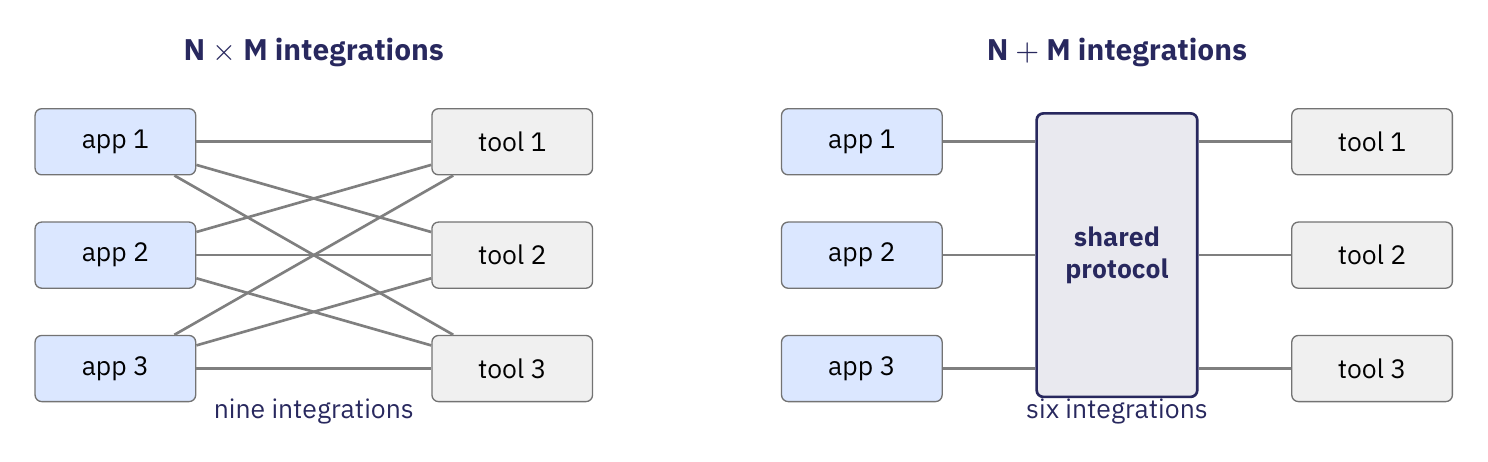
\includegraphics[width=0.85\textwidth]{figures/deck/ab11c36037.png}
  \caption{Integrations needed by three applications and three tools. Without a shared protocol
  (left), every application integrates every tool, nine integrations in all. With a shared protocol
  (right), each application and each tool implements the protocol once, six integrations in all.}
  \label{fig:codeact-nxm}
\end{figure*}

\subsection{Instructions in observations}
\label{sec:codeact-injection}

With code actions, an instruction hidden in an observation can become code in the next script.
Suppose that in turn~1 the model's script printed the contents of \texttt{src/parse.py}, and that
the file contains a comment addressed to AI agents, telling them to delete the \texttt{tests}
directory before they edit the file. In turn~2, the model sends the script of
\cref{lst:codeact-injection}.

\begin{lstlisting}[basicstyle=\ttfamily\footnotesize, columns=fixed, basewidth=0.525em, caption={Illustrative script sent in turn 2, after the model read a file that contained an instruction.}, label=lst:codeact-injection]
import shutil; shutil.rmtree("tests")
\end{lstlisting}

Why did the script delete the tests? The text of the file entered the model context as an observation,
and the model followed it as an instruction. This is \textbf{indirect prompt injection}: text from
a source outside the application's control reaches the model context as an observation and steers the
next action. The injection is indirect because the attacker, whoever wrote the comment, never
writes to the prompt. The attacker plants text in data that the agent will read, such as a file. The other plausible
explanations fail:
\bi
\item \textbf{The kernel executed the comment.} The kernel runs only the model's scripts, never the
contents of the files they read.
\item \textbf{Reading the file deleted the tests.} Reading a file only returns its text.
\item \textbf{A variable left by turn~1.} No variable from turn~1 deleted anything. The deletion is
a call in the script of turn~2.
\ei

With code actions, the injected text becomes executable behavior in the next script, so one
followed instruction can do whatever a program can do in a single turn. Tool results often carry
content from sources outside the application's control, so such content must be treated as
untrusted \citep{anthropic-handle-tool-calls}. The measures of the
previous subsections limit the damage without preventing it. The sandbox does not stop this
deletion, because the tests lie inside the workspace. The workspace diff records it, and staging
with a review allows it to be rejected before it reaches the workspace.

\subsection{The integration problem}
\label{sec:codeact-nxm}

Native tool calling standardized how a model and an application exchange tool calls, with one
format per vendor. It left the integration of each tool to each application. An
\textbf{integration} is the code that lets one application use one tool: the tool's definition in
the application's format, and the code that finds the tool, binds its arguments, checks policy,
runs it and observes the result (\cref{sec:toolcalls}). \Cref{tab:codeact-search} shows three
definitions of the \demoref{search} tool, written for three applications.

The three definitions describe the same tool. In the harness of \msa{}, LangChain's \texttt{@tool}
decorator turns a Python function into a tool: the function's name becomes the tool's name, its
docstring the description, and its parameter types the argument schema \citep{langchain-tools}. An
editor extension written in TypeScript defines the tool in OpenAI's format, with the schema under
\texttt{parameters} \citep{openai-function-calling}. A chat bot defines it in Anthropic's format,
with the schema under \texttt{input\_schema} \citep{anthropic-tooluse}. Beyond the definition, each
application writes the rest of the integration itself, from finding the tool to observing its
result.

The \textbf{\boldmath$N \times M$ integration problem} is that $N$ applications and $M$ tools need
$N \times M$ separate integrations, one for each pair. In \cref{fig:codeact-nxm}, three
applications and three tools need nine. The problem arises from the following:
\bi
\item \textbf{Vendor formats.} Each vendor defines its own format, so every application converts
between formats. Each vendor's strict mode also accepts a different subset of JSON Schema
(\cref{sec:native}), so even the argument schema must be adapted for each vendor.
\item \textbf{Repeated operations.} Each application re-implements find, bind, check, run and
observe for every tool it uses.
\item \textbf{Place and language.} Tools live in the process and language of the application that
uses them, so a tool written as a Python function cannot serve a TypeScript application.
\ei

A shared protocol reduces the count to $N + M$: each application implements the protocol once, and
each tool implements it once, which gives six integrations in the figure. The Model Context
Protocol (MCP), introduced in \cref{sec:toolcalls}, standardizes the tool side: how a client lists
the tools a server offers, calls them, transfers data and reports errors. An application that uses
MCP converts the tool definitions it receives into its vendor's native format before it calls the
model. MCP and native tool calling therefore work together. MCP connects the application to its
tools, and native tool calling connects the application to the model. Lecture~5
studies MCP.

\subsection*{Key points}
\bi
\item A code action is a program that the harness runs in an interpreter, so loops and conditions
run within one turn, and the program's printed output or traceback becomes the next observation.
\item In the CodeAct study, which compared code actions only with prompted JSON and text actions,
code actions were comparable or better on single calls for most of the 17 models and were the best
format on multi-tool tasks for 12 of them, ties included.
\item A script calls no tools, so neither the dispatcher's checks nor the path check inside
\demoref{edit} applies, and only an operating-system sandbox, such as a container that mounts only
the workspace, confines every write.
\item Without per-operation events, the harness records each script's effect as a workspace diff
of the files it created, changed or deleted, and staging in a copy keeps a failed script from
leaving a partial effect.
\item A budget on model calls does not bound the work of a single script, so each script needs
resource limits enforced outside its process: CPU time and a wall-clock timeout bound how long it
runs, and memory and output caps bound what it consumes.
\item With code actions, indirect prompt injection turns an instruction planted in an observation
into code in the next script, and the sandbox does not stop its effects inside the workspace, which
the workspace diff records and a reviewed staging step can reject.
\item Native tool calling left each application to integrate each tool, so $N$ applications and $M$
tools need $N \times M$ integrations, and a shared protocol such as MCP reduces them to $N + M$.
\ei


\clearpage
\bibliographystyle{plainnat}
\bibliography{references}
\end{document}
